%==============================================================================
% The Syndrome Algebra for Differentiable Parametric Systems
% From a Discrete Quantum Error-Correcting Codes to the Continuous Limit
%
% A pure-mathematics companion paper to \cite{ThreeModesLLM}.
% Generalises the [[5,1,3]] quantum error-correcting code to the
% continuous real-valued regime, arriving at S = N(J-bar . V)^T.
%
% Target length: 22-26 pages.
%==============================================================================

\documentclass[11pt,a4paper]{article}

\usepackage[utf8]{inputenc}
\usepackage[T1]{fontenc}
\usepackage{amsmath,amssymb,amsthm,mathtools}
\usepackage{geometry}
\usepackage{booktabs}
\usepackage{array}
\usepackage{xcolor}
\usepackage{hyperref}
\usepackage{enumitem}
\usepackage{float}
\usepackage[most]{tcolorbox}
\usepackage{tikz}
\usepackage{pgfplots}
\usepackage{orcidlink}
\usepackage{todonotes}
\pgfplotsset{compat=1.17}
\usetikzlibrary{positioning,arrows.meta,calc,matrix,decorations.pathreplacing}

\geometry{margin=1.15in}

\hypersetup{
  colorlinks=true,
  linkcolor=blue!70!black,
  citecolor=blue!60!black,
  urlcolor=blue!60!black
}

%--- Colours ------------------------------------------------------------------
\definecolor{defbg}{RGB}{240,244,255}
\definecolor{defclr}{RGB}{50,80,160}
\definecolor{thmbg}{RGB}{240,255,240}
\definecolor{thmclr}{RGB}{30,120,30}
\definecolor{corbg}{RGB}{255,248,225}
\definecolor{corclr}{RGB}{150,100,10}
\definecolor{notebg}{RGB}{252,252,245}
\definecolor{noteclr}{RGB}{100,100,60}
\definecolor{mode1col}{RGB}{180,50,50}    % Mode 1 red
\definecolor{mode2col}{RGB}{50,80,180}    % Mode 2 blue
\definecolor{mode3col}{RGB}{50,180,80}    % Mode 3 green

\newtcolorbox{defbox}[1][]{colback=defbg,colframe=defclr!80!black,
  fonttitle=\bfseries\sffamily,title={#1},breakable,enhanced,
  boxrule=1pt,left=6pt,right=6pt}
\newtcolorbox{thmbox}[1][]{colback=thmbg,colframe=thmclr!80!black,
  fonttitle=\bfseries\sffamily,title={#1},breakable,enhanced,
  boxrule=1.2pt,left=6pt,right=6pt}
\newtcolorbox{corbox}[1][]{colback=corbg,colframe=corclr!80!black,
  fonttitle=\bfseries\sffamily,title={#1},breakable,enhanced,
  boxrule=1pt,left=6pt,right=6pt}
\newtcolorbox{notebox}[1][]{colback=notebg,colframe=noteclr!70!black,
  fonttitle=\bfseries\sffamily,title={#1},breakable,enhanced,
  boxrule=0.8pt,left=6pt,right=6pt}

%--- Theorem environments -----------------------------------------------------
\newtheorem{theorem}{Theorem}[section]
\newtheorem{lemma}[theorem]{Lemma}
\newtheorem{corollary}[theorem]{Corollary}
\newtheorem{proposition}[theorem]{Proposition}
\theoremstyle{definition}
\newtheorem{definition}[theorem]{Definition}
\newtheorem{remark}[theorem]{Remark}

%--- Macros -------------------------------------------------------------------
\newcommand{\Wm}{\mathbf{W}}
\newcommand{\Gm}{\mathbf{G}}
\newcommand{\Um}{\mathbf{U}}
\newcommand{\Vm}{\mathbf{V}}
\newcommand{\Sm}{\mathbf{S}}
\newcommand{\Jm}{\mathbf{J}}
\newcommand{\Hm}{\mathbf{H}}
\newcommand{\Imat}{\mathbf{I}}
\newcommand{\Sig}{\boldsymbol{\Sigma}}
\newcommand{\vk}[1][]{\mathbf{v}_{#1}}
\newcommand{\uk}[1][]{\mathbf{u}_{#1}}
\newcommand{\sk}[1][]{\mathbf{s}_{#1}}
\newcommand{\ek}[1][]{\mathbf{e}_{#1}}
\newcommand{\onevec}{\mathbf{1}}
\newcommand{\Rbb}{\mathbb{R}}
\newcommand{\Fbb}{\mathbb{F}}
\newcommand{\Nop}{\mathcal{N}}
\newcommand{\Xop}{\hat{X}}
\newcommand{\Pop}{\hat{P}}
\newcommand{\Aop}{\hat{A}}
\newcommand{\Bop}{\hat{B}}
\newcommand{\Eop}{\mathbb{E}}
\newcommand{\norm}[1]{\left\lVert#1\right\rVert}
\newcommand{\inner}[2]{\left\langle#1,\,#2\right\rangle}
\newcommand{\floor}[1]{\left\lfloor#1\right\rfloor}
\newcommand{\dstar}{\delta^{*}}
\newcommand{\dimin}{d_{\mathrm{in}}}
\newcommand{\dimout}{d_{\mathrm{out}}}
\newcommand{\Cnumber}{\mathbb{C}}

%==============================================================================
\title{%
  \textbf{The Syndrome Algebra \\for Differentiable Parametric Systems}\\[0.4em]
  \large From a Discrete Quantum Error-Correcting Codes to the Continuous Limit
}
\author{Marek Hubka\, \orcidlink{0009-0003-2476-9017}
  \thanks{Independent Researcher, Czech Republic.\\
    Email: \href{mailto:marek@tidesofuncertainty.com}{marek@tidesofuncertainty.com}}}
\date{May 2026}
%==============================================================================

\begin{document}
\maketitle

\begin{abstract}
We address a diagnostic question that has no satisfactory answer in the literature: given a differentiable parametric system whose internal state is unobservable, how can one identify, from outputs alone, which component of the internal state was perturbed, by how much, and in which direction? The classical answer for linear systems is the parity-check matrix; for quantum systems it is the stabilizer syndrome. This paper gives the answer for any differentiable parametric system whose parameters live in a real finite Hilbert space.

Starting from the $[\![5,1,3]\!]_2$ perfect quantum error-correcting code --- which encodes one logical qubit in five physical qubits, corrects any single-qubit error, and saturates the quantum Singleton bound --- we identify three structural replacements that carry the construction into the continuous real-valued regime: the finite field $\Fbb_q$ is replaced by $\Rbb$, the Pauli error basis by the singular-value decomposition basis of the parameter map, and the parity-check map by the averaged Jacobian. Under these replacements, the syndrome table becomes the matrix
\[
\Sm \;=\; \Nop\!\left(\bar{\Jm}\cdot\Vm\right)^{\!\top}
\]
in which $\bar{\Jm}$ is the averaged Jacobian, $\Vm$ is the matrix of right singular vectors, and $\Nop$ denotes row-wise $\ell_2$ normalisation. We prove that this is the $q\to\infty$ limit of the discrete syndrome table, that the $[\![5,1,3]\!]_2$ code is recovered as the binary special case at $q=2$, and we establish four immediate properties of the algebra together with two uncertainty principles that govern measurement precision and architectural capacity. The present paper is concerned only with the mathematics; application and experimental validation of the algebra on a particular class of probabilistic systems is in the companion paper~\cite{ThreeModesLLM}.
\end{abstract}

\newpage
\tableofcontents
\newpage

%==============================================================================
\section{Introduction}
\label{sec:intro}
%==============================================================================

\subsection{The Diagnostic Problem for Probabilistic Systems}
\label{sec:intro_problem}

Let
\begin{equation}
  f: \Theta \times \mathcal{X} \;\longrightarrow\; \mathcal{P}(\mathcal{Y})
  \label{eq:bb_intro}
\end{equation}
be a differentiable map, where $\mathcal{X}$ is an input space, $\mathcal{Y}$ is a finite output alphabet of size $q = |\mathcal{Y}|$, $\mathcal{P}(\mathcal{Y})$ is the probability simplex over $\mathcal{Y}$, and $\Theta \subset \Rbb^n$ is a finite-dimensional real Hilbert space of parameters. The internal state $\theta\in\Theta$ is unobservable: the analyst sees only the output distribution $f(x;\theta)\in\mathcal{P}(\mathcal{Y})$ for chosen probe inputs $x\in\mathcal{X}$.

Suppose the parameters undergo an unknown perturbation $\theta \mapsto \theta + \Delta\theta$ which alters the output distribution. The diagnostic question is threefold:
\begin{enumerate}[nosep,label=(\roman*)]
  \item Which component of $\theta$ was perturbed?
  \item By how much?
  \item In which direction within the relevant parameter subspace?
\end{enumerate}
For linear systems the answer is supplied by the parity-check matrix: the syndrome $\sk = \Hm\ek$ identifies the error pattern $\ek$ modulo the kernel of $\Hm$. For quantum systems the answer is supplied by the stabilizer formalism: each stabilizer generator yields one syndrome bit, and the syndrome table maps each correctable error to a unique bit pattern. In both cases the syndrome computation is linear over a finite field and the lookup is exact.

The intermediate regime --- continuous, probabilistic, high-dimensional, with differentiable parameter dependence --- has not been given a unified mathematical treatment. The present paper shows that the coding-theoretic structure is intact in this regime, but only after three simultaneous replacements have been understood.

\subsection{The Coding-Theoretic Starting Point}
\label{sec:intro_start}

The concrete anchor is the $[\![5,1,3]\!]_2$ quantum error-correcting (QEC) code~\cite{Laflamme1996, Bennett1996, Knill1997}. It encodes one logical qubit into five physical qubits, corrects any single-qubit error (bit flip, phase flip, or both), and saturates the quantum Singleton bound~\cite{Singleton1964, Ekert1996} $k \leq n - 2(d-1)$. Its four stabilizer generators generate an abelian group of $16$ elements, and the corresponding parity-check matrix $\Hm\in\Fbb_2^{4\times 10}$ maps each of the $15$ single-qubit error operators (and the identity) to a unique $4$-bit syndrome.

The question this paper asks is: \emph{what is this construction when the alphabet is $\Rbb$ rather than $\Fbb_2$?} The discrete code relies on properties of the Pauli group, the symplectic form on $\Fbb_2^{2n}$, and modular arithmetic. None of these objects survives verbatim in the continuous setting. What does survive --- and what this paper makes precise --- is the underlying algebraic skeleton: a parity-check map taking error operators to syndrome signatures, an orthonormal error basis intrinsic to the system, and a lookup operation that is a maximisation of inner product.

\paragraph{One application, then nothing more.}
The mathematics developed below has an unexpected application to neural network diagnostics, where weight matrix perturbations play the role of errors and changes in the output logit distribution play the role of syndromes. That application is validated experimentally in the companion paper~\cite{ThreeModesLLM}; the present paper is concerned only with the mathematics, and the reader is not assumed to know anything about neural networks.

\paragraph{What the algebra does.}
The construction was designed for exactly the class of problem set out in \S\ref{sec:intro_problem}: systems whose internal state is not directly observable. In the quantum case the encoded logical state is inaccessible by hypothesis --- a measurement that read it would collapse the encoding. The syndrome measurement circumvents this by coupling the unobservable interior to observable ancilla qubits through the commutation structure of the error operators~\cite{NielsenChuang2000, Gottesman1997, Laflamme1996, Bennett1996, Knill1997}; what the ancillas reveal is not the encoded state but the error \emph{relative} to it, read from the boundary. Information is extracted from inaccessible dimensions not by observing them directly, but by reading their fingerprint in the observable boundary. The continuous generalisation developed below extends this principle without weakening it. The null space of the Gram metric~(\ref{def:gram}) --- the span of right singular directions $v_k$ with $\sigma_k \to 0$ --- plays the role of the unobservable interior: those directions received no gradient signal and produce no observable output change on in-distribution inputs. The probe sequences play the role of the ancilla qubits, and the syndrome table $\Sm \;=\; \Nop\!\left(\bar{\Jm}\cdot\Vm\right)^{\!\top}$ is the instrument that couples the invisible geometry to the observable boundary. The algebra's reach into the unobservable is not an accidental feature of one application; it is what the construction was for from the beginning. \emph{The syndrome algebra was designed, from its quantum origins, to extract structure from dimensions that cannot be observed directly.}

\subsection{Structure of the Paper}
\label{sec:intro_structure}

Section~\ref{sec:513} works the $[\![5,1,3]\!]_2$ code completely: all sixteen syndrome entries computed by hand, the measurement protocol, and the q-dependence of the Singleton bound. Section~\ref{sec:replacements} introduces the three replacements that carry the construction into the continuous regime. Section~\ref{sec:syndrome_table} establishes the syndrome algebra formally and proves the main equation $\Sm = \Nop(\bar{\Jm}\cdot\Vm)^\top$. Section~\ref{sec:properties} proves four immediate properties of the algebra (oracle correction, crossing error, the null space interpretation, and multi-layer identifiability). Section~\ref{sec:up} establishes two uncertainty principles, one at the level of measurement and one at the level of architecture. Appendix~\ref{app:correspondence} gives the complete correspondence between the discrete and continuous structures. Appendix~\ref{app:worked} works the same numerical example through both the discrete and continuous formalisms in parallel.

%==============================================================================
\section{The \texorpdfstring{$[\![5,1,3]\!]_2$}{[[5,1,3]]} Code}
\label{sec:513}
%==============================================================================

\subsection{Setup: Five Qubits, One Logical Qubit}
\label{sec:513_setup}

The physical Hilbert space is $\mathcal{H} = (\Cnumber^2)^{\otimes 5}$, the tensor product of five qubit spaces, where $\Cnumber$ denotes the complex numbers. A single Pauli operator acting on one qubit is one of
\[
  I = \begin{pmatrix}1&0\\0&1\end{pmatrix},\quad
  X = \begin{pmatrix}0&1\\1&0\end{pmatrix},\quad
  Z = \begin{pmatrix}1&0\\0&-1\end{pmatrix},\quad
  Y = iXZ.
\]
The Pauli group on $n$ qubits is the set of tensor products of these single-qubit operators with phases in $\{\pm 1,\pm i\}$.

The $[\![5,1,3]\!]_2$ code is the simultaneous $+1$ eigenspace $\mathcal{C}\subset\mathcal{H}$ of four commuting Pauli operators called \emph{stabilizer generators}:
\begin{equation}
\begin{aligned}
  g_1 &= X \otimes Z \otimes Z \otimes X \otimes I, \\
  g_2 &= I \otimes X \otimes Z \otimes Z \otimes X, \\
  g_3 &= X \otimes I \otimes X \otimes Z \otimes Z, \\
  g_4 &= Z \otimes X \otimes I \otimes X \otimes Z.
\end{aligned}
\label{eq:gens}
\end{equation}
These generate an abelian subgroup $\mathcal{G}$ of order $|\mathcal{G}| = 2^4 = 16$, and $\mathcal{C}$ is two-dimensional, encoding one logical qubit: $\dim(\mathcal{H}) = 32$, the stabilizer cuts the dimension in half four times.

\subsection{The Parity-Check Matrix}
\label{sec:513_pc}

The standard symplectic representation maps Pauli strings on $n$ qubits to vectors in $\Fbb_2^{2n}$. A Pauli string $P = P_1\otimes\cdots\otimes P_n$ is represented as $(a\,|\,b)\in
\Fbb_2^{2n}$ with
\[
  a_j = \begin{cases}1 & P_j\in\{X,Y\}\\ 0 & \text{else}\end{cases}
  \qquad
  b_j = \begin{cases}1 & P_j\in\{Z,Y\}\\ 0 & \text{else}\end{cases}
\]
Two Pauli strings $P=(a\,|\,b)$, $P'=(a'\,|\,b')$ commute iff $a\cdot b' + b\cdot a' = 0\pmod 2$. The single-qubit Paulis at position $j$ then have representations $X_j=(\ek[j]\,|\,\mathbf{0})$, $Z_j=(\mathbf{0}\,|\,\ek[j])$, and $Y_j=(\ek[j]\,|\,\ek[j])$, where $\ek[j]\in\Fbb_2^5$ is the standard basis vector.

The four stabilizer generators of $[[5,1,3]]$ code~\eqref{eq:gens} give the rows of a $4\times 10$ matrix $\Hm$ over $\Fbb_2$, with the first five columns indexing the $X$-part and the last five indexing the $Z$-part. The syndrome of an error $\ek=(a\,|\,b)\in\Fbb_2^{10}$ is
\begin{equation}
  \sk \;=\; \Hm\,\ek \pmod 2 \;\in\; \Fbb_2^4 .
  \label{eq:hsyndrome}
\end{equation}
For our generators, the rows of $\Hm$ are read off from~ $[[5,1,3]]$ code~\eqref{eq:gens} by recording, in each of the five positions, whether the generator carries $X$ (contributing to the $X$-part) and whether it carries $Z$ (contributing to the $Z$-part). Direct computation gives
\begin{equation}
  \Hm \;=\; \left[\,\Hm_X\;\Big|\;\Hm_Z\,\right] \;=\;
  \left[\begin{array}{ccccc|ccccc}
    1 & 0 & 0 & 1 & 0 & 0 & 1 & 1 & 0 & 0 \\
    0 & 1 & 0 & 0 & 1 & 0 & 0 & 1 & 1 & 0 \\
    1 & 0 & 1 & 0 & 0 & 0 & 0 & 0 & 1 & 1 \\
    0 & 1 & 0 & 1 & 0 & 1 & 0 & 0 & 0 & 1
  \end{array}\right]
  \label{eq:hmatrix}
\end{equation}
where row $i$ records $g_i$. Equivalently, the syndrome bit $s_i = (\Hm\ek)_i$ is $1$ iff the error $\ek$ anticommutes with $g_i$.

\subsection{The Syndrome Table: All Sixteen Entries}
\label{sec:513_table}

There are $15$ non-trivial single-qubit error operators ($X_j$, $Y_j$, $Z_j$ for $j=1,\dots,5$) and the identity, giving $16$ total errors. There are $2^4 = 16$ syndrome patterns. Because the $[\![5,1,3]\!]_2$ code is perfect, the map error~$\mapsto$~syndrome is a bijection.

The syndrome of a Pauli error $E$ with symplectic vector $(a_e|b_e)$ against a stabilizer generator $g_i$ with vector $(a_{g_i}|b_{g_i})$ is the symplectic pairing
\begin{equation}
  s_i \;=\; a_e\cdot b_{g_i} \;+\; b_e \cdot a_{g_i} \pmod 2 ,
  \label{eq:symplectic_rule}
\end{equation}
which equals $1$ exactly when $E$ and $g_i$ anticommute. In practice: $X_j$ anticommutes with $g_i$ iff $g_i$ carries a $Z$ at position $j$; $Z_j$ anticommutes with $g_i$ iff $g_i$ carries an $X$ at position $j$; and $Y_j$ syndrome is the bitwise sum of the $X_j$ and $Z_j$ syndromes. Applying~\eqref{eq:symplectic_rule} to the generators of~\eqref{eq:gens} and collecting the four bits $s_1 s_2 s_3 s_4$ for every single-qubit error gives Table~\ref{tab:syndromes513}.

\begin{table}[h]
\centering
\renewcommand{\arraystretch}{1.15}
\begin{tabular}{l c c | l c c | l c c}
\toprule
\textbf{Error} & $s_1s_2s_3s_4$ & \texttt{bits} &
\textbf{Error} & $s_1s_2s_3s_4$ & \texttt{bits} &
\textbf{Error} & $s_1s_2s_3s_4$ & \texttt{bits} \\
\midrule
& & & $I$ & $0\,0\,0\,0$ & \texttt{0000} & & & \\
\midrule
$X_1$  & $0\,0\,0\,1$ & \texttt{0001} &
$Y_1$  & $1\,0\,1\,1$ & \texttt{1011} &
$Z_1$  & $1\,0\,1\,0$ & \texttt{1010} \\
$X_2$  & $1\,0\,0\,0$ & \texttt{1000} &
$Y_2$  & $1\,1\,0\,1$ & \texttt{1101} &
$Z_2$  & $0\,1\,0\,1$ & \texttt{0101} \\
$X_3$  & $1\,1\,0\,0$ & \texttt{1100} &
$Y_3$  & $1\,1\,1\,0$ & \texttt{1110} &
$Z_3$  & $0\,0\,1\,0$ & \texttt{0010} \\
$X_4$  & $0\,1\,1\,0$ & \texttt{0110} &
$Y_4$  & $1\,1\,1\,1$ & \texttt{1111} &
$Z_4$  & $1\,0\,0\,1$ & \texttt{1001} \\
$X_5$  & $0\,0\,1\,1$ & \texttt{0011} &
$Y_5$  & $0\,1\,1\,1$ & \texttt{0111} &
$Z_5$  & $0\,1\,0\,0$ & \texttt{0100} \\
\bottomrule
\end{tabular}
\caption{The complete $[\![5,1,3]\!]_2$ syndrome table. The $15$ single-qubit errors and the identity give a bijection with the $16$ patterns $\Fbb_2^4$.}
\label{tab:syndromes513}
\end{table}

A graphical representation appears in Figure~\ref{fig:syn_grid}.

\begin{figure}[h]
\centering
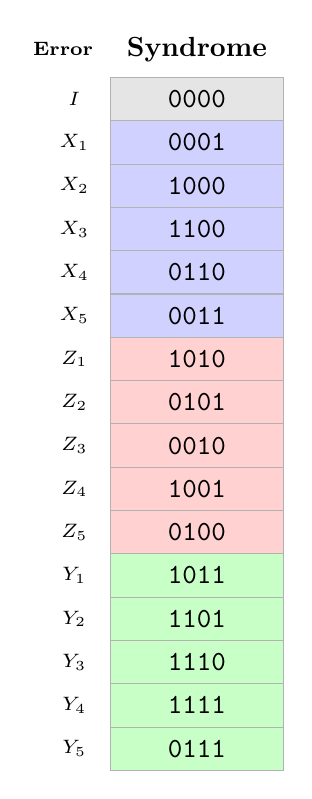
\begin{tikzpicture}[
  cellh/.style={minimum width=2.2cm,minimum height=0.55cm,inner sep=0pt},
  labelh/.style={minimum width=0.9cm,minimum height=0.55cm,inner sep=0pt,font=\scriptsize}
]
  \node[labelh,anchor=south] at (0,0.35) {\textbf{Error}};
  \node[cellh,anchor=south] at (1.7,0.35) {\textbf{Syndrome}};
  % rows: y, label, syndrome, color
  \foreach \y/\lbl/\synd/\col in {%
     0/$I$/{0000}/{gray!20},
    -1/$X_1$/{0001}/{blue!18},
    -2/$X_2$/{1000}/{blue!18},
    -3/$X_3$/{1100}/{blue!18},
    -4/$X_4$/{0110}/{blue!18},
    -5/$X_5$/{0011}/{blue!18},
    -6/$Z_1$/{1010}/{red!18},
    -7/$Z_2$/{0101}/{red!18},
    -8/$Z_3$/{0010}/{red!18},
    -9/$Z_4$/{1001}/{red!18},
    -10/$Z_5$/{0100}/{red!18},
    -11/$Y_1$/{1011}/{green!22},
    -12/$Y_2$/{1101}/{green!22},
    -13/$Y_3$/{1110}/{green!22},
    -14/$Y_4$/{1111}/{green!22},
    -15/$Y_5$/{0111}/{green!22}%
  }{
    \node[labelh,anchor=east] at (0.6,\y*0.55) {\lbl};
    \node[cellh,fill=\col,draw=black!30] at (1.7,\y*0.55) {\texttt{\synd}};
  }
\end{tikzpicture}
\caption{The $[\![5,1,3]\!]_2$ syndrome table. Identity (grey), $X$-errors (blue), $Z$-errors (red), $Y$-errors (green). All $16$ bit patterns are realised exactly once.}
\label{fig:syn_grid}
\end{figure}

\subsection{Syndrome Measurement and Correction}
\label{sec:513_meas}

The diagnostic protocol uses an ancilla qubit attached to each stabilizer generator, prepared in a controlled state, and measured after the unitary $g_i$ is applied controlled on the ancilla. The outcome is $+1$ if the encoded state commutes with $g_i$ and $-1$ if it anticommutes. Encoding outcomes as bits, the four measurements
yield a syndrome vector $\sk\in\Fbb_2^4$. The procedure is:
\begin{enumerate}[nosep]
  \item Measure each of the four generators $g_1,\dots,g_4$ on the received state, recording outcomes as $\pm 1$.
  \item Translate the outcomes to bits ($+1\mapsto 0$, $-1\mapsto 1$) to obtain $\sk\in\Fbb_2^4$.
  \item Look up $\sk$ in Table~\ref{tab:syndromes513} to identify the error $E\in\{I,X_j,Y_j,Z_j\}$.
  \item Apply $E$ to the received state. Since every single-qubit Pauli is its own inverse, this restores the original encoded state exactly.
\end{enumerate}

\begin{notebox}[The ancilla measurement]
The stabilizer measurements commute with the logical operators of the code. Hence the measurement does not disturb the encoded information: it extracts only the syndrome, which is information \emph{about the error}, not about the encoded state. This is the property that makes coherent quantum diagnostics possible without back-action, and it is the property that the continuous syndrome algebra will inherit in a modified form.
\end{notebox}

\subsection{The Singleton Bound and \texorpdfstring{$q$}{q}-Dependence}
\label{sec:513_singleton}

For a quantum stabilizer code $[\![n,k,d]\!]_q$ encoding $k$ logical qudits into $n$ physical qudits over alphabet $\Fbb_q$, the quantum Singleton bound is
\begin{equation}
  k \;\leq\; n - 2(d-1).
  \label{eq:singleton}
\end{equation}
A code that saturates~\eqref{eq:singleton} is called quantum maximum distance separable (MDS). For the $[\![5,1,3]\!]_2$ code, $1 = 5 - 2(3-1) = 1$: the bound is saturated.

The Pauli group generalises to the Heisenberg--Weyl~\cite{Knill1997} group $\mathcal{HW}_q$ over $\Fbb_q$, generated by operators $X(a)$ and $Z(b)$ for $a,b\in\Fbb_q$ with relation $Z(b)X(a) = \omega^{ab}X(a)Z(b)$, $\omega = e^{2\pi i/q}$. The symplectic representation of $\mathcal{HW}_q$ takes values in $\Fbb_q^{2n}$. The syndrome of an error $\ek\in\Fbb_q^{2n}$ is $\sk = \Hm \ek$ with $\Hm \in\Fbb_q^{m\times 2n}$, $m = n-k$.

The maximum normalised distance $\delta_{\max} = d_{\max}/n$ satisfies, by the Singleton bound,
\begin{equation}
  \delta_{\max} \;=\; \frac{q^2 - 1}{q^2}
  \;=\; 1 - \frac{1}{q^2}.
  \label{eq:dmax}
\end{equation}
As $q$ grows, $\delta_{\max}\to 1$: the alphabet grows, the syndrome table can resolve finer error patterns, and the correctable fraction of the parameter space approaches unity.

The natural question is:
\begin{center}
\emph{What is this construction in the limit $q\to\infty$?}
\end{center}
This question is the subject of the next section.

%==============================================================================
\section{Three Replacements}
\label{sec:replacements}
%==============================================================================

The passage from the discrete code over $\Fbb_q$ to the continuous algebra over $\Rbb$ requires three structural replacements applied \emph{simultaneously}. Each is forced by the demand that the limiting object retain the diagnostic properties of the discrete code: an orthonormal error basis, a linear parity-check map, and a syndrome lookup operation.

We fix notational conventions for the remainder of the paper. Indices follow these classes:
\begin{itemize}[nosep]
  \item $a, b$: output indices, ranging over $1,\dots,q$.
  \item $\mu, \nu$: input parameter indices, ranging over
    $1,\dots,\dimin$.
  \item $k$: SVD direction index, ranging over $1,\dots,r$.
  \item $i$: probe input index, ranging over $1,\dots,n_p$.
\end{itemize}
We adopt the Einstein summation convention for repeated indices within the same expression unless otherwise noted.

\subsection{Replacement 1: \texorpdfstring{$\Fbb_q \to \Rbb$}{F\_q to R}}
\label{sec:rep1}

The finite field $\Fbb_q$ is naturally embedded in $\Rbb$ for any prime power $q$, identifying $\{0,1,\ldots,q-1\}$ with the corresponding integers. As $q\to\infty$, the set $\{0,1,\ldots,q-1\}\subset\Rbb$ becomes dense in $[0,q-1]\subset\Rbb$. After rescaling by $q$, it becomes dense in $[0,1]$. Modular arithmetic becomes ordinary arithmetic in the limit (the modulus disappears as the field becomes large enough that ``wraparound'' never occurs for bounded error magnitudes).

Formally, the syndrome alphabet $\Fbb_q^m$ becomes $\Rbb^m$. The syndrome computation, which was a matrix-vector product mod $q$, becomes a matrix-vector product over $\Rbb$. The lookup operation, which was bitstring equality, must be replaced by something continuous: maximisation of inner product (cosine matching) is the natural choice.

\begin{notebox}[Why cosine matching]
In $\Fbb_2$, syndromes either match or they do not: equality is binary. In $\Rbb$, syndromes generically do not match exactly, but they have well-defined inner products. The inner product $\inner{\sk}{\sk'}/(\norm{\sk}\norm{\sk'})$ is the cosine of the angle between two unit vectors in $\Rbb^m$. Cosine matching reduces to bitstring equality when the syndromes are restricted to $\{0,1\}^m$ and the inner product is computed mod $2$. It is the unique scale-invariant generalisation.
\end{notebox}

The relation $\delta_{\max} = 1 - q^{-2}$ from~\eqref{eq:dmax} has limit $\delta_{\max}\to 1$ as $q\to\infty$. The full unit interval of normalised distances is achieved.

\subsection{Replacement 2: Pauli Basis \texorpdfstring{$\to$}{to} SVD Basis}
\label{sec:rep2}

This is the deepest of the three replacements and the only one that requires construction of new mathematical content, not merely extension by limit.

In the discrete case, the Pauli operators $\{X_j, Z_j, Y_j\}$ form the canonical error basis because they are orthonormal under the Hilbert--Schmidt inner product $\inner{P}{Q} = \frac{1}{2^n}\mathrm{tr}(P^\dagger Q)$ and they diagonalise the symplectic form on $\Fbb_q^{2n}$ (each pair anticommutes with one other Pauli at the same position and commutes with all others). They are intrinsic to the system: not chosen by the analyst, but determined by the algebraic structure of the ambient group.

In the continuous case, we seek the analogous canonical basis for perturbations of a real parameter map. Let $\Wm \in \Rbb^{\dimout \times \dimin}$ be a weight matrix --- one block of the parameter vector --- and consider perturbations $\Delta\Wm$ of this matrix.

\begin{defbox}[Definition --- Gram metric]
\begin{definition}
\label{def:gram}
The \emph{Gram matrix} of $\Wm$ is
\begin{equation}
  \Gm = \Wm^\top \Wm \in \Rbb^{\dimin\times\dimin},
  \qquad
  G_{\mu\nu} = W^a{}_\mu W_{a\nu}.
  \label{eq:gram}
\end{equation}
$\Gm$ is symmetric positive semi-definite~\cite{Horn2012}: it defines a Riemannian metric on the input parameter subspace, the metric induced on $\Rbb^{\dimin}$ by the linear map $\Wm$.
The term \emph{Gram matrix} refers to the same object in linear algebra; we adopt \emph{Gram metric} to emphasise its geometric role.
\end{definition}
\end{defbox}

The spectral decomposition of $\Gm$ is the singular value decomposition~\cite{Horn2012} of $\Wm$. Write
\begin{equation}
  \Wm = \Um\Sig\Vm^\top, \qquad
  \Um\in\Rbb^{\dimout\times r},\;
  \Sig = \mathrm{diag}(\sigma_1\geq\cdots\geq\sigma_r),\;
  \Vm\in\Rbb^{\dimin\times r},
  \label{eq:svd}
\end{equation}
where $r = \min(\dimout,\dimin)$, $\Um^\top\Um = \Vm^\top\Vm = \Imat_r$, and the singular values $\sigma_k\geq 0$ are ordered decreasingly. Then
\begin{equation}
  \Gm = \Vm\Sig^2\Vm^\top,
  \qquad
  G_{\mu\nu}v_k{}^\nu = \sigma_k{}^2\, v_k{}^\mu .
  \label{eq:gram_spec}
\end{equation}
The columns $\vk[1],\ldots,\vk[r]$ of $\Vm$ are the eigenvectors of $\Gm$ --- the right singular vectors of $\Wm$. They are orthonormal in the standard inner product on $\Rbb^{\dimin}$ and they diagonalise $\Gm$.

\paragraph{The key claim.}
The SVD directions $\{\vk[k]\}$ are the continuous analogue of the Pauli basis. The correspondence is structural and exact:

\begin{itemize}[nosep]
  \item Both are orthonormal bases: $\inner{\vk[j]}{\vk[k]} = \delta_{jk}$ in $\Rbb^{\dimin}$, $\inner{P_j}{P_k}_{HS} = \delta_{jk}$ on operators.
  \item Both diagonalise the natural metric on the error space: the symplectic form in the discrete case, the Gram metric in the continuous case.
  \item Both are intrinsic to the system: the Pauli basis is fixed by the Pauli group structure; the SVD basis is fixed by the map $\Wm$ itself.
  \item Neither basis is chosen by the analyst.
\end{itemize}
This is summarised in the commutative diagram of Figure~\ref{fig:commutative}.

\begin{figure}[h]
\centering
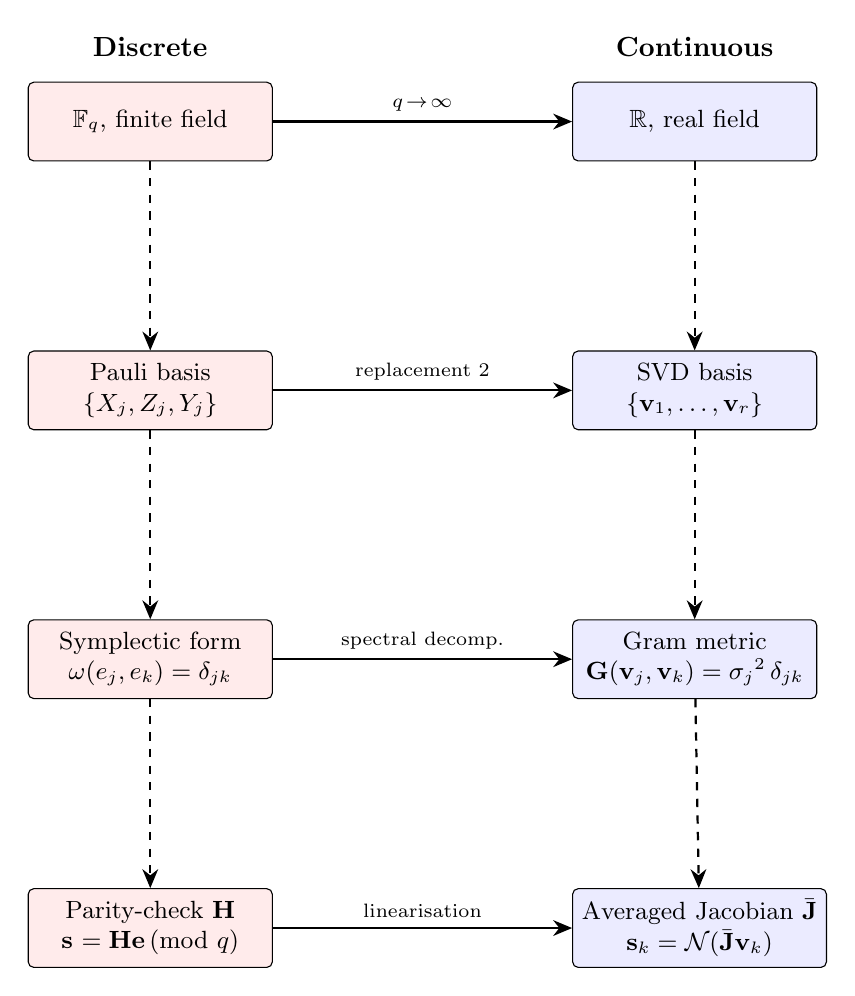
\begin{tikzpicture}[node distance=2.4cm and 3.8cm,
                    box/.style={draw,rounded corners=2pt,
                                minimum width=3.1cm,minimum height=1cm,
                                align=center,font=\small},
                    bar/.style={-{Stealth[length=2.4mm,width=2mm]},thick}]

  \node[box,fill=red!8]   (Fq)   {$\Fbb_q$, finite field};
  \node[box,fill=red!8,below=of Fq]   (Pauli){Pauli basis\\$\{X_j,Z_j,Y_j\}$};
  \node[box,fill=red!8,below=of Pauli](Symp) {Symplectic form\\$\omega(e_j,e_k) = \delta_{jk}$};
  \node[box,fill=red!8,below=of Symp](Hmd)  {Parity-check $\Hm$\\$\sk = \Hm\ek\!\!\pmod q$};

  \node[box,fill=blue!8,right=of Fq]    (Rb)   {$\Rbb$, real field};
  \node[box,fill=blue!8,right=of Pauli] (SVD)  {SVD basis\\$\{\vk[1],\ldots,\vk[r]\}$};
  \node[box,fill=blue!8,right=of Symp]  (Gm)   {Gram metric\\$\Gm(\vk[j],\vk[k]) = \sigma_j{}^2\,\delta_{jk}$};
  \node[box,fill=blue!8,right=of Hmd]   (Jb)   {Averaged Jacobian $\bar{\Jm}$\\$\sk[k] = \Nop(\bar{\Jm}\vk[k])$};

  \draw[bar] (Fq)    -- node[above,font=\scriptsize]{$q\!\to\!\infty$} (Rb);
  \draw[bar] (Pauli) -- node[above,font=\scriptsize]{replacement 2} (SVD);
  \draw[bar] (Symp)  -- node[above,font=\scriptsize]{spectral decomp.} (Gm);
  \draw[bar] (Hmd)   -- node[above,font=\scriptsize]{linearisation} (Jb);

  \draw[bar,dashed] (Fq) -- (Pauli);
  \draw[bar,dashed] (Pauli) -- (Symp);
  \draw[bar,dashed] (Symp) -- (Hmd);
  \draw[bar,dashed] (Rb) -- (SVD);
  \draw[bar,dashed] (SVD) -- (Gm);
  \draw[bar,dashed] (Gm) -- (Jb);

  \node[draw=none,above=0.2cm of Fq,font=\bfseries]{Discrete};
  \node[draw=none,above=0.2cm of Rb,font=\bfseries]{Continuous};
\end{tikzpicture}
\caption{Three replacements. Vertical arrows: the discrete and continuous formalisms each build their syndrome computation from field, error basis, and pairing form. Horizontal arrows: the three replacements that connect them.}
\label{fig:commutative}
\end{figure}

\paragraph{Geometric content.}
Definition~\ref{def:gram} carries geometric content that the Pauli analogy alone does not capture. The Gram metric is \emph{elliptical}: different SVD directions have different curvatures $\sigma_k{}^2$, which are generically unequal. Directions with $\sigma_k$ large correspond to perturbations that produce large output changes (``signal''); directions with $\sigma_k\approx 0$ correspond to perturbations that produce no output change on the manifold spanned by the columns of $\Wm^\top$ (``null'').

In the Pauli basis, this distinction does not exist: every Pauli operator is treated equally by the symplectic form. The continuous-case basis carries extra information --- the magnitudes $\{\sigma_k\}$ --- that distinguishes structurally different error directions. This information will be essential in Section~\ref{sec:properties} when we identify the null space as the confabulation subspace.

\subsection{Replacement 3: Parity-Check Map \texorpdfstring{$\to$}{to} Jacobian}
\label{sec:rep3}

It remains to identify the continuous counterpart of the parity-check matrix $\Hm$. We require a linear map taking errors (perturbations of $\Wm$) to syndromes (changes in the output distribution).

For a weight matrix $\Wm = \Um\Sig\Vm^\top$, the canonical \emph{rank-one SVD-aligned perturbation} in direction $k$ is
\begin{equation}
  \Delta\Wm_k(\varepsilon) \;=\; \varepsilon\, \uk[k]\, \vk[k]^\top
  \;\in\; \Rbb^{\dimout \times \dimin},
  \label{eq:err_op}
\end{equation}
where $\uk[k]\in\Rbb^{\dimout}$ and $\vk[k]\in\Rbb^{\dimin}$ are the $k$-th left and right singular vectors of $\Wm$.\footnote{Equivalently, $\Wm + \Delta\Wm_k(\varepsilon) = \Um(\Sig + \varepsilon\Eop_{kk})\Vm^\top$ where $\Eop_{kk}$ has a single $1$ in position $(k,k)$: the perturbation shifts the $k$-th singular value by $\varepsilon$ and leaves all other singular values and singular vectors unchanged.} This is the natural continuous counterpart of the symplectic basis of single-qubit Paulis: each $\Delta\Wm_k$ targets one ``coordinate'' of the parameter space adapted to $\Wm$.

Let $\ell: \mathcal{X}\times\Theta \to \Rbb^q$ be a logit function, i.e.\ a function whose row-wise softmax is the output distribution $f(x;\theta)$ of~\eqref{eq:bb_intro}. We will work throughout with logits, since they carry the same information as the probability distribution but are unconstrained by the simplex.

The change in logit at input $x$ due to perturbation $\Delta\Wm_k(\varepsilon)$ is
\begin{equation}
  \boldsymbol{\delta}_k(x,\varepsilon)
  \;=\; \ell(x;\, \theta + \Delta\Wm_k(\varepsilon))
       - \ell(x;\, \theta).
  \label{eq:delta_def}
\end{equation}
By differentiability and the chain rule, for small $\varepsilon$,
\begin{equation}
  \boldsymbol{\delta}_k(x,\varepsilon)
  \;=\; \varepsilon\, \Jm(x)\cdot \vk[k] \;+\; O(\varepsilon^2),
  \label{eq:taylor1}
\end{equation}
where $\Jm(x) \in \Rbb^{q\times\dimin}$ is the Jacobian of the logit with respect to $\Wm$ at input $x$. In index notation, with $a$ ranging over output components and $\mu$ over input parameter directions:
\begin{equation}
  J(x)^a{}_\mu \;=\; \frac{\partial \ell^a(x;\theta)}
                          {\partial W^a{}_\mu} \;+\; \text{contractions}
  ,\qquad
  J(x)\vk[k] \;=\;
  \sum_{a,\mu,b}
   u_k{}^b \frac{\partial \ell^a(x;\theta)}{\partial W^b{}_\mu}\, v_k{}^\mu\,\boldsymbol{e}_a ,
  \label{eq:jacobian_def}
\end{equation}
where $\boldsymbol{e}_a$ is the standard basis of $\Rbb^q$. The contraction with the rank-one tensor $\uk[k]\vk[k]^\top$ in the parameter index pair $(b,\mu)$ collapses to a single output-space vector $\Jm(x)\vk[k]\in\Rbb^q$.

Now average over $n_p$ probe inputs $\{x_1,\dots,x_{n_p}\}$:
\begin{equation}
  \bar{\boldsymbol{\delta}}_k(\varepsilon)
  \;\coloneqq\; \frac{1}{n_p}\sum_{i=1}^{n_p}
                \boldsymbol{\delta}_k(x_i,\varepsilon)
  \;=\; \varepsilon\, \bar{\Jm}\cdot\vk[k] \;+\; O(\varepsilon^2),
  \label{eq:avg_delta}
\end{equation}
with $\bar{\Jm} = n_p^{-1}\sum_i \Jm(x_i)$ the averaged Jacobian. Normalising to a unit vector gives the syndrome:
\begin{equation}
  \sk[k] \;=\; \Nop\!\left(\bar{\boldsymbol{\delta}}_k(\varepsilon)\right)
        \;=\; \Nop(\bar{\Jm}\cdot\vk[k]) \;\in\; \Rbb^q,
        \quad \norm{\sk[k]} = 1,
  \label{eq:sk_def}
\end{equation}
where $\Nop(\boldsymbol{w}) = \boldsymbol{w}/\norm{\boldsymbol{w}}$ is $\ell_2$ normalisation. The normalisation is the continuous analogue of taking residues mod~$q$: it removes the magnitude of the perturbation, retaining only its direction in syndrome space.

\paragraph{The connection.}
The averaged Jacobian $\bar{\Jm}$ plays exactly the role of $\Hm$. The map $\vk[k]\mapsto \bar{\Jm}\vk[k]$ is the continuous analogue of $\ek\mapsto \Hm\ek$. The normalisation $\Nop$ is the continuous analogue of the modular reduction $\pmod q$.

\subsection{The Limit \texorpdfstring{$q\to\infty$}{q to infinity}}
\label{sec:rep_limit}

Collecting the three replacements:
\begin{center}
\renewcommand{\arraystretch}{1.35}
\begin{tabular}{lll}
\toprule
\textbf{Discrete} & \textbf{Continuous} & \textbf{Replacement} \\
\midrule
$\Fbb_q$ (finite field) & $\Rbb$ (real field) & 1 \\
Pauli operators $\{X_j,Z_j,Y_j\}$ & SVD directions $\{\vk[k]\}$ & 2 \\
Parity-check matrix $\Hm$ & Averaged Jacobian $\bar{\Jm}$ & 3 \\
Modular arithmetic $\pmod q$ & $\ell_2$ normalisation $\Nop$ & 1 \\
Bitstring equality lookup & Cosine maximisation lookup & 1 \\
$\delta_{\max} = 1 - q^{-2}$ & $\delta_{\max} = 1$ & 1 \\
\bottomrule
\end{tabular}
\end{center}

Stacking the syndromes $\sk[k]$ as the rows of a matrix
$\Sm\in\Rbb^{r\times q}$ yields, by~\eqref{eq:sk_def},
\begin{equation}
  \boxed{\;\Sm \;=\; \Nop\!\left(\bar{\Jm}\cdot\Vm\right)^\top\;}
  \label{eq:main}
\end{equation}
This is the syndrome table of the continuous algebra. The next section formalises this construction as a definition and proves that~\eqref{eq:main} is the $q\to\infty$ limit of the discrete construction --- with the $[\![5,1,3]\!]_2$ code recovered as the $q=2$ binary special case.

%==============================================================================
\section{The Continuous Syndrome Table}
\label{sec:syndrome_table}
%==============================================================================

We now state the construction formally, then prove the main equation.

\subsection{The Probabilistic Black Box}
\label{sec:bb}
\begin{defbox}[Definition --- Probabilistic black box]
\begin{definition}
\label{def:bb}
A \emph{probabilistic black box} is a tuple $(f, \Theta, \mathcal{X}, \mathcal{Y})$ with $\mathcal{X}$ an input space, $\mathcal{Y}$ a finite output alphabet of size $q$, $\Theta \subset \Rbb^n$ a parameter space partitioned as $\theta = (\Wm_1, \ldots,\Wm_L)$ into $L$ weight matrices, and
\[
  f: \mathcal{X}\times\Theta \to \mathcal{P}(\mathcal{Y})
\]
a map differentiable in $\theta$. The associated \emph{logit map} $\ell: \mathcal{X}\times\Theta \to \Rbb^q$ has $f$ as its softmax and is differentiable in $\theta$.
\end{definition}
\end{defbox}

The partition of $\theta$ into weight matrices is the structural assumption that makes the syndrome algebra non-trivial. For a generic differentiable map without such a partition the construction applies to the single weight matrix $\theta\in\Rbb^n$ regarded as a row vector; for systems with multiple matrices each weight matrix carries its own SVD basis, its own Gram metric, and its own syndrome table.

\subsection{The Gram Metric and Its Spectral Decomposition}
\label{sec:gram_metric}

\begin{defbox}[Definition --- SVD basis and signal/null decomposition]
\begin{definition}
\label{def:signal_null}
Let $\Wm\in\Rbb^{\dimout\times\dimin}$ be a weight matrix with SVD $\Wm = \Um\Sig\Vm^\top$ as in~\eqref{eq:svd}, and let $\sigma_{\mathrm{thresh}}\geq 0$ be a fixed numerical threshold.

The \emph{signal space} of $\Wm$ is
\[
  \mathcal{S}(\Wm) \;=\; \mathrm{span}\{\vk[k] : \sigma_k > \sigma_{\mathrm{thresh}}\},
\]
and the \emph{null space} is
\[
  \mathcal{N}(\Wm) \;=\; \mathrm{span}\{\vk[k] : \sigma_k \leq \sigma_{\mathrm{thresh}}\}.
\]
The \emph{stable rank} is
$\mathrm{SR}(\Wm) = \sum_k \sigma_k{}^2 / \sigma_1{}^2$ and the
\emph{dimensional excess} is
$\mathrm{DE}(\Wm) = \dimin / \mathrm{SR}(\Wm) \geq 1$.
\end{definition}
\end{defbox}

The signal space carries the structured response of $\Wm$ to perturbations; the null space carries directions in which $\Wm$ acts trivially. In the discrete case, no analogue of this split exists, because every Pauli direction is equally significant under the symplectic form. In the continuous case the split is fundamental.

\subsection{Error Operators and Syndromes}
\label{sec:errs_syns}

\begin{defbox}[Definition --- Error operator]
\begin{definition}
\label{def:error_op}
For weight matrix $\Wm = \Um\Sig\Vm^\top$ with SVD basis $\{\vk[k]\}_{k=1}^{r}$ on input side and $\{\uk[k]\}_{k=1}^{r}$ on output side, the \emph{error operator} in direction $k$ at magnitude $\varepsilon > 0$ is the rank-one SVD-aligned perturbation
\begin{equation}
  \Delta\Wm_k(\varepsilon) \;=\; \varepsilon\,\uk[k]\,\vk[k]^\top
  \;\in\; \Rbb^{\dimout\times\dimin}.
  \label{eq:err_op_def}
\end{equation}
The collection $\{\Delta\Wm_k(\varepsilon)\}_{k=1}^{r}$ is the \emph{error basis} at magnitude $\varepsilon$.
\end{definition}
\end{defbox}

\begin{defbox}[Definition --- Syndrome and syndrome table]
\begin{definition}
\label{def:syndrome}
Given a probe set $\{x_i\}_{i=1}^{n_p}\subset\mathcal{X}$, the \emph{syndrome} of error direction $k$ at magnitude $\varepsilon$ is
\begin{equation}
  \sk[k](\varepsilon)
  \;=\; \Nop\!\left(
    \frac{1}{n_p}\sum_{i=1}^{n_p}
    \bigl[\ell(x_i; \theta + \Delta\Wm_k(\varepsilon))
           -\ell(x_i;\theta)\bigr]
  \right) \;\in\; \Rbb^q .
  \label{eq:syndrome_def}
\end{equation}
The \emph{syndrome table} is the matrix $\Sm\in\Rbb^{r\times q}$ with rows $\sk[k]^\top$.
\end{definition}
\end{defbox}

The syndrome $\sk[k]$ is a unit vector by construction. The syndrome table $\Sm$ has orthonormal columns of $\Vm$ as its row labels and the output coordinates $a\in\{1,\ldots,q\}$ as its column labels.

\subsection{Theorem 1: The Jacobian Is the Syndrome Table}
\label{sec:thm1}

\begin{thmbox}[Theorem 1 --- The Jacobian is the syndrome table]
\begin{theorem}
\label{thm:main}
Let $(f, \Theta, \mathcal{X}, \mathcal{Y})$ be a probabilistic black box as in Definition~\ref{def:bb}. Let $\Wm$ be one of its weight matrices with SVD $\Wm = \Um\Sig\Vm^\top$. Let $\bar{\Jm} = n_p^{-1} \sum_i \Jm(x_i) \in \Rbb^{q\times\dimin}$ be the averaged Jacobian of the logit output with respect to $\Wm$ evaluated at the probe set $\{x_i\}_{i=1}^{n_p}$. Then in the limit $\varepsilon\to 0$ (equivalently, to first order in $\varepsilon$):
\begin{equation}
  \Sm \;=\; \Nop\!\left(\bar{\Jm}\cdot \Vm\right)^\top
  \;\in\;\Rbb^{r\times q},
  \label{eq:main_thm}
\end{equation} 
where $\Nop$ denotes row-wise $\ell_2$ normalisation. Row $k$ of $\Sm$ is the syndrome $\sk[k]$ of the $k$-th SVD direction.
\end{theorem}
\end{thmbox}

\begin{proof}
The proof proceeds in four steps.

\noindent\emph{Step 1 (definition).}
By Definition~\ref{def:syndrome},
\[
  \sk[k](\varepsilon) \;=\;
  \Nop\!\left(
    \frac{1}{n_p}\sum_{i=1}^{n_p}
    \bigl[\ell(x_i; \theta + \Delta\Wm_k(\varepsilon))
           -\ell(x_i;\theta)\bigr]
  \right).
\]

\noindent\emph{Step 2 (Taylor expansion).}
Since $\ell$ is differentiable in $\theta$, for each fixed $x_i$ and each $k\in\{1,\ldots,r\}$ there exists a Jacobian $\Jm(x_i) \in \Rbb^{q\times\dimin}$ such that, for $\varepsilon$ in a neighbourhood of $0$,
\begin{equation}
  \ell^a(x_i; \theta + \Delta\Wm_k(\varepsilon))
  - \ell^a(x_i;\theta)
  \;=\; \varepsilon\, J(x_i)^a{}_\mu v_k{}^\mu \;+\; R^a(x_i, \varepsilon),
  \label{eq:proof_taylor}
\end{equation}
where the remainder satisfies $|R^a(x_i,\varepsilon)| \leq C \varepsilon^2$ for some constant $C = C(x_i, \theta)$, uniformly in $a$. In matrix form, $\ell(x_i; \theta + \Delta\Wm_k(\varepsilon)) - \ell(x_i;\theta) = \varepsilon \Jm(x_i)\vk[k] + O(\varepsilon^2)$.

\noindent\emph{Step 3 (averaging).}
Substituting~\eqref{eq:proof_taylor} into Step~1 and using linearity of the average,
\begin{align}
  \frac{1}{n_p}\sum_{i=1}^{n_p}
  \bigl[\ell(x_i; \theta + \Delta\Wm_k(\varepsilon))
         -\ell(x_i;\theta)\bigr]
  &\;=\; \varepsilon\,\bar{\Jm}\,\vk[k] \;+\;
        \frac{1}{n_p}\sum_{i=1}^{n_p} \boldsymbol{R}(x_i,\varepsilon) \notag\\
  &\;=\; \varepsilon\,\bar{\Jm}\,\vk[k] \;+\; O(\varepsilon^2).
  \label{eq:proof_avg}
\end{align}

\noindent\emph{Step 4 (normalisation and stacking).}
The normalisation $\Nop$ is positively homogeneous of degree zero: $\Nop(\lambda\boldsymbol{w}) = \Nop(\boldsymbol{w})$ for all $\lambda > 0$. Dividing inside~\eqref{eq:proof_avg} by $\varepsilon > 0$ before applying $\Nop$ and taking $\varepsilon\to 0^+$,
\begin{equation}
  \sk[k]
  \;=\; \lim_{\varepsilon\to 0^+}
        \Nop\!\left(
          \frac{1}{n_p\,\varepsilon}\!\!
          \sum_{i=1}^{n_p}\!
          \bigl[\ell(x_i;\theta + \Delta\Wm_k(\varepsilon))-\ell(x_i;\theta)\bigr]
        \right)
  \;=\; \Nop\!\left(\bar{\Jm}\,\vk[k]\right) .
  \label{eq:proof_limit}
\end{equation}
The matrix $\bar{\Jm}\Vm \in \Rbb^{q\times r}$ has columns $\bar{\Jm}\vk[k]$. Its row-wise normalisation followed by transpose gives a matrix whose $k$-th row is $\Nop(\bar{\Jm}\vk[k])^\top = \sk[k]^\top$. Stacking these rows yields
\[
  \Sm \;=\; \Nop\!\left(\bar{\Jm}\cdot\Vm\right)^\top.
  \qedhere
\]
\end{proof}

\begin{remark}
\label{rmk:513_special}
The $[\![5,1,3]\!]_2$ code is recovered from~\eqref{eq:main_thm} by the substitutions
\[
  q = 2, \qquad \bar{\Jm} \;\rightsquigarrow\; \Hm \pmod 2,
  \qquad \Vm \;\rightsquigarrow\; \Imat_{10},
  \qquad \Nop \;\rightsquigarrow\; \mathrm{id}.
\]
Under these substitutions, $\Sm = (\Hm \cdot \Imat_{10})^\top \pmod 2 = \Hm^\top$, and the syndrome of the $k$-th error is the $k$-th column of $\Hm$. This recovers Table~\ref{tab:syndromes513} exactly; the parallel computation is worked through in Appendix~\ref{app:worked}.
\end{remark}

\begin{figure}[h]
\centering
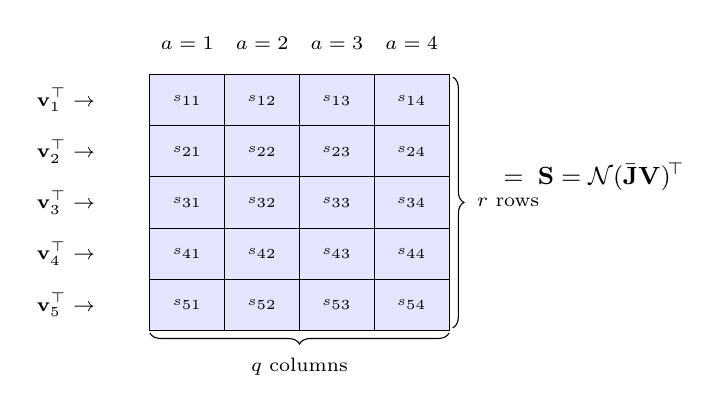
\begin{tikzpicture}[x=0.95cm,y=0.65cm]
  % Row labels
  \foreach \i in {1,...,5}{
    \node[anchor=east,font=\scriptsize] at (0.4,-\i+0.5) {$\vk[\i]^\top\to$};
  }
  % Column heads
  \foreach \j in {1,...,4}{
    \node[anchor=south,font=\scriptsize] at (\j+0.5,0.3) {$a=\j$};
  }
  % Matrix entries
  \foreach \i in {1,...,5}{
    \foreach \j in {1,...,4}{
      \draw[fill=blue!10] (\j,-\i+1) rectangle (\j+1,-\i);
      \node[font=\tiny] at (\j+0.5,-\i+0.5) {$s_{\i\j}$};
    }
  }
  \node[anchor=west,font=\small] at (5.6,-2) {$=\;\Sm
                                              = \Nop(\bar{\Jm}\Vm)^{\!\top}$};
  \draw[decorate,decoration={brace,amplitude=4pt,mirror}]
        (5.05,-5+0.05) -- (5.05,0-0.05)
        node[midway,xshift=20pt,font=\scriptsize] {$r$ rows};
  \draw[decorate,decoration={brace,amplitude=4pt,mirror}]
        (1,-5.05) -- (5,-5.05)
        node[midway,yshift=-12pt,font=\scriptsize] {$q$ columns};
\end{tikzpicture}
\caption{The continuous syndrome table $\Sm$ as a labelled matrix. Each row $\sk[k]^\top$ is the unit-norm syndrome of the $k$-th SVD direction. Compare with the discrete table from Figure~\ref{fig:syn_grid}: there $r=10$ rows, $q=4$ columns of binary entries; here $r$ rows, $q$ columns of real entries.}
\label{fig:syn_table}
\end{figure}

%==============================================================================
\section{Properties of the Algebra}
\label{sec:properties}
%==============================================================================

We now establish four immediate properties of the syndrome algebra: oracle correction is exact on the linear path, correction in the wrong direction always harms output, the null space of the Gram metric is the subspace of undetectable errors, and multi-layer measurement (in systems with $L>1$) achieves full identifiability.

\subsection{Theorem 2: Oracle Correction Is Exact on the Linear Path}
\label{sec:oracle}

\begin{thmbox}[Theorem 2 --- Oracle correction]
\begin{theorem}
\label{thm:oracle}
Let $\Wm \mapsto \Wm + \Delta\Wm_k(\varepsilon)$ be an error operator applied to the parameter space. If the error direction $k$ and the magnitude $\varepsilon$ are known exactly, then the inverse perturbation $\Wm\mapsto\Wm - \Delta\Wm_k(\varepsilon)$ restores the original parameter exactly: the residual $\norm{\ell(x;\Wm_{\mathrm{corrected}}) - \ell(x;\Wm)} = 0$ for every $x\in\mathcal{X}$.
\end{theorem}
\end{thmbox}

\begin{proof}
By definition of the error operator,
\[
  \Wm_{\mathrm{perturbed}} \;=\; \Wm + \varepsilon\uk[k]\vk[k]^\top.
\]
Applying the inverse perturbation,
\[
  \Wm_{\mathrm{corrected}}
  \;=\; \Wm_{\mathrm{perturbed}} - \varepsilon\uk[k]\vk[k]^\top
  \;=\; \Wm + \varepsilon\uk[k]\vk[k]^\top - \varepsilon\uk[k]\vk[k]^\top
  \;=\; \Wm.
\]
The map $f$ depends on $\theta$ only through its current value, not through any history, so for every input $x$ the output distribution $f(x;\theta_{\mathrm{corrected}}) = f(x;\theta)$, and likewise for the logit. Hence $\norm{\ell(x;\Wm_{\mathrm{corrected}}) - \ell(x;\Wm)} = 0$.
\end{proof}

\begin{remark}
\label{rmk:no_linearity}
Theorem~\ref{thm:oracle} does not require linearity of $f$ in $\theta$. The correction is exact because the parameter is the state, and restoring the state is arithmetic. The role of linearity in subsequent theorems is to relate the syndrome (an output-space quantity) to the parameter perturbation (a parameter-space quantity); for the correction itself, no linearity assumption is needed once the perturbation is identified.
\end{remark}

\subsection{Theorem 3: Crossing Error Is Always Positive}
\label{sec:crossing}

\begin{thmbox}[Theorem 3 --- Crossing error]
\begin{theorem}
\label{thm:crossing}
Suppose the system is perturbed in direction $\vk[k^*]$ (true error) with magnitude $\varepsilon$, and correction is then applied in direction $\vk[j]\neq\vk[k^*]$ with magnitude $\varepsilon^*$ (estimated from the observed perturbation). Assume that $\bar{\Jm}$ has full column rank on the signal space of $\Wm$, and that the images $\bar{\Jm}\vk[k^*]$ and $\bar{\Jm}\vk[j]$ are orthogonal in $\Rbb^q$.\footnote{For an exactly linear logit $\ell(x;\Wm) = \Wm x$, the SVD-aligned error operator gives $\bar{\Jm}\vk[k] = c_k \uk[k]$ where $c_k = \tfrac{1}{n_p}\sum_i \vk[k]^\top x_i$, so the images $\bar{\Jm}\vk[k]$ are scalar multiples of the orthonormal left singular vectors $\{\uk[k]\}$ and the orthogonality hypothesis is automatic. For non-linear $\ell$ the hypothesis is the structural condition that the averaged Jacobian preserves the orthogonality of the SVD basis under image; see Appendix~\ref{app:worked} for a concrete instance.} Then to first order in the perturbation magnitudes,
\begin{equation}
\begin{split}
  \Eop_x\!\left[\norm{\ell(x;\Wm_{\mathrm{wrong}}) - \ell(x;\Wm)}^2\right]
  &\;=\; \varepsilon^2 \norm{\bar{\Jm}\vk[k^*]}^2
        + (\varepsilon^*)^2 \norm{\bar{\Jm}\vk[j]}^2 \\
  & \qquad\;>\; \Eop_x\!\left[\norm{\ell(x;\Wm_{\mathrm{perturbed}})
        - \ell(x;\Wm)}^2\right].
\end{split}
\label{eq:crossing}
\end{equation}
The squared residual after wrong correction strictly exceeds the squared residual before correction.
\end{theorem}
\end{thmbox}

\begin{proof}
By Theorem~\ref{thm:main}, the expected first-order change in $\ell$ from the perturbation $\Delta\Wm_{k^*}(\varepsilon)$ is $\varepsilon\bar{\Jm}\vk[k^*]$, and the expected first-order change from the wrong correction $-\varepsilon^*\uk[j]\vk[j]^\top$ is $-\varepsilon^*\bar{\Jm}\vk[j]$. By linearity, the net expected change is
\[
  \Eop_x[\ell(x;\Wm_{\mathrm{wrong}}) - \ell(x;\Wm)]
  \;=\; \varepsilon\bar{\Jm}\vk[k^*] - \varepsilon^*\bar{\Jm}\vk[j].
\]
The expected squared norm is
\begin{align*}
  \norm{\varepsilon\bar{\Jm}\vk[k^*] - \varepsilon^*\bar{\Jm}\vk[j]}^2
  &= \varepsilon^2 \norm{\bar{\Jm}\vk[k^*]}^2
   - 2\varepsilon\varepsilon^* \inner{\bar{\Jm}\vk[k^*]}{\bar{\Jm}\vk[j]}
   + (\varepsilon^*)^2 \norm{\bar{\Jm}\vk[j]}^2 \\
  &= \varepsilon^2 \norm{\bar{\Jm}\vk[k^*]}^2
   + (\varepsilon^*)^2 \norm{\bar{\Jm}\vk[j]}^2,
\end{align*}
the cross term vanishing by the orthogonality hypothesis. The right-hand side strictly exceeds $\varepsilon^2 \norm{\bar{\Jm}\vk[k^*]}^2$ whenever $\varepsilon^* > 0$ and $\bar{\Jm}\vk[j] \neq 0$ (signal direction $j$). The crossing error
\[
  \Delta \;=\; (\varepsilon^*)^2\norm{\bar{\Jm}\vk[j]}^2
  \;>\; 0
\]
is strictly positive.
\end{proof}

\begin{remark}
\label{rmk:expectation}
The proof works in expectation over probe inputs because the $O(\varepsilon^2)$ remainders of Theorem~\ref{thm:main} are input-dependent. For a single input $x$, the local Jacobian $\Jm(x)$ may deviate from $\bar{\Jm}$, and the per-input squared residual may temporarily decrease. The deviation of $\Jm(x)$ from $\bar{\Jm}$ across inputs is quantified by the Jacobian variance $V_j$ of Section~\ref{sec:up}, which is the obstruction to exact syndrome identification.
\end{remark}

\subsection{Theorem 4: The Null Space Is the Confabulation Subspace}
\label{sec:null}

\begin{thmbox}[Theorem 4 --- Null space invariance]
\begin{theorem}
\label{thm:null}
Let $\vk[k]$ be an SVD direction of $\Wm$ with singular value $\sigma_k = 0$, and let $\mathcal{X}_{\mathrm{in}}\subset\mathcal{X}$ be the support of the input distribution on which $\Wm$ was trained (i.e.\ for which the rows of $\Wm$ are linear combinations of input features). Then:
\begin{enumerate}[label=(\alph*),nosep]
  \item For all $x\in\mathcal{X}_{\mathrm{in}}$, $\Jm(x)\vk[k] = 0$. Consequently $\bar{\Jm}\vk[k] = 0$ and the syndrome $\sk[k]$ is undefined (the normalisation $\Nop(\mathbf{0})$ is degenerate).
  \item For $x\in\mathcal{X}\setminus\mathcal{X}_{\mathrm{in}}$, $\Jm(x)\vk[k]$ is unconstrained: it can take any value in $\Rbb^q$.
\end{enumerate}
\end{theorem}
\end{thmbox}

\begin{proof}
\emph{(a)} The Gram metric $\Gm = \Wm^\top\Wm$ has eigenvalues $\sigma_k{}^2$. When $\sigma_k = 0$, $\vk[k] \in \ker(\Wm)$, since $\norm{\Wm\vk[k]}^2 = \vk[k]^\top\Gm\vk[k] = \sigma_k{}^2 = 0$. For any input $x$ whose pre-activation feature vector lies in the column span of $\Wm^\top$ (the in-distribution condition), the contribution of direction $\vk[k]$ to the output is identically zero --- the parameter direction is unused on the trained input manifold. By differentiation, $\Jm(x)\vk[k] = 0$ for all such $x$, and averaging gives $\bar{\Jm}\vk[k] = 0$.

\emph{(b)} For inputs $x$ outside $\mathcal{X}_{\mathrm{in}}$, the feature vector need not lie in the column span of $\Wm^\top$. The constraint $\Jm(x)\vk[k] = 0$ then no longer follows from the training of $\Wm$; the null direction retains its full geometric freedom. Concrete examples in which $\Jm(x)\vk[k]\neq 0$ for out-of-distribution $x$ are constructed in companion paper~\cite{ThreeModesLLM}.
\end{proof}

\begin{notebox}[Interpretation]
A perturbation in a null direction produces no syndrome on the trained input manifold (it is invisible to diagnostic measurement), but produces unconstrained output changes on novel inputs. This is the precise statement of what is sometimes called confabulation: the system has free behavioural latitude in directions that the training data could not constrain.
\end{notebox}

\subsection{Theorem 5: Multi-Layer Measurement Achieves Identifiability}
\label{sec:multi_layer}

When the parameter space has $L > 1$ weight matrices and the probabilistic black box has a layered structure (the output of layer $\ell$ is the input of layer $\ell+1$), the syndrome algebra extends naturally: each layer provides one syndrome table. A perturbation introduced at layer $k^*$ propagates through the subsequent layers and produces a sequence of residual changes $\bar{\boldsymbol{\delta}}^{(L)}_{k^*}$ at each downstream layer $L\geq k^*$.

\begin{defbox}[Definition --- Causal localisation]
\begin{definition}
\label{def:causal}
For a perturbation $\Delta\Wm_{k^*}^{(j)}(\varepsilon)$ injected at weight matrix $k^*$ in SVD direction $j$, the \emph{residual stream change} at layer $L$ is
\[
  \bar{\boldsymbol{\delta}}_L \;=\;
  \Eop_x\bigl[ r_L(x;\theta + \Delta\Wm_{k^*}^{(j)}(\varepsilon))
              - r_L(x;\theta) \bigr],
\]
where $r_L(x;\theta) \in \Rbb^{d_L}$ is the activation at the output of layer $L$. For acyclic computation graphs:
\[
  \norm{\bar{\boldsymbol{\delta}}_L} = 0 \quad\text{for}\quad L < k^*,
  \qquad
  \norm{\bar{\boldsymbol{\delta}}_L} > 0 \quad\text{for}\quad L \geq k^* .
\]
The transition identifies the originating layer $k^*$ exactly.
\end{definition}
\end{defbox}

\begin{thmbox}[Theorem 5 --- Multi-layer identifiability]
\begin{theorem}
\label{thm:multilayer}
Consider a probabilistic black box with $L$ weight matrices, and a perturbation at weight matrix $k^*$ in SVD direction $j\in\{1,\ldots,r\}$. Define:
\begin{itemize}[nosep]
  \item \emph{Single-layer syndrome:} $\sk[j]^{(\mathrm{log})} = \Nop(\bar{\Jm}_{\mathrm{log}}\vk[j]^{(k^*)}) \in \Rbb^q$, the syndrome at the logit (output) level only.
  \item \emph{Multi-layer syndrome:} the concatenation $\mathbf{m}_j = (\bar{\boldsymbol{\delta}}_{k^*}, \ldots, \bar{\boldsymbol{\delta}}_L, \sk[j]^{(\mathrm{log})}) \in \Rbb^{D_*}$ with $D_* = \sum_{L\geq k^*} d_L + q$.
\end{itemize}
Suppose there exist two distinct directions $j, j'$ with $\sk[j]^{(\mathrm{log})} = \sk[j']^{(\mathrm{log})}$ (single-layer confusion). For generic weight matrices, if $D_* \geq r$ then $\mathbf{m}_j \neq \mathbf{m}_{j'}$: the multi-layer syndrome distinguishes them.
\end{theorem}
\end{thmbox}

\begin{proof}
Two directions $\vk[j],\vk[j']$ with equal single-layer syndromes have $\bar{\Jm}_{\mathrm{log}}\vk[j]$ parallel to $\bar{\Jm}_{\mathrm{log}}\vk[j']$. Their difference lies in the kernel of $\bar{\Jm}_{\mathrm{log}}$ (after a scalar rescaling), hence in an at most $(\dimin - q)$-dimensional subspace of $\Rbb^{\dimin}$.

The multi-layer syndrome appends $\sum_{L\geq k^*} d_L$ additional real-valued coordinates, one per layer. Each downstream layer's Jacobian to the residual stream is a linear map $\Jm^{(L)}: \Rbb^{\dimin} \to \Rbb^{d_L}$. Generically these maps are not all parallel: their joint kernel
\[
  \bigcap_{L\geq k^*}\ker(\Jm^{(L)}) \cap \ker(\bar{\Jm}_{\mathrm{log}})
\]
is generically of codimension at least $D_*$ in $\Rbb^{\dimin}$.

If $D_* \geq r$, the joint kernel intersects the SVD basis trivially (zero-dimensionally), and no two SVD directions are mapped to the same multi-layer syndrome. The multi-layer measurement is identifiability-complete.
\end{proof}

\begin{remark}
Theorem~\ref{thm:multilayer} mirrors the role of multiple stabilizer generators in the discrete code. The $[\![5,1,3]\!]_2$ code has four generators because one or two would not suffice to distinguish all $15$ single-qubit errors; the same dimensional argument applies here. Each additional layer is one additional stabilizer measurement, and the total syndrome lives in a product space whose dimension grows linearly with the number of layers.
\end{remark}

%==============================================================================
\section{Two Uncertainty Principles}
\label{sec:up}
%==============================================================================

The syndrome algebra exhibits two distinct uncertainty principles. The first, the Jacobian Uncertainty Principle (JUP), is a \emph{measurement} uncertainty: it bounds the precision with which a syndrome can be identified given a finite probe set, in terms of an intrinsic property of the SVD direction (the Jacobian variance). The second, the Reliability Principle (RP), is an \emph{architectural} uncertainty: it relates the three normalised coordinates of a coding-theoretic system (distance, capacity, slack) by a simplex constraint and an AM-GM inequality.

\subsection{Jacobian Variance}
\label{sec:jvar}

\begin{defbox}[Definition --- Jacobian variance]
\begin{definition}
\label{def:jv}
For SVD direction $\vk[k]$ and probe set $\{x_1,\ldots,x_{n_p}\}$, the \emph{Jacobian variance} is
\begin{equation}
  V_k \;=\; \frac{1}{n_p}\sum_{i=1}^{n_p}
          \norm{\Jm(x_i)\vk[k] - \bar{\Jm}\vk[k]}^2 .
  \label{eq:jvar}
\end{equation}
\end{definition}
\end{defbox}

$V_k$ measures the input-dependence of the syndrome: how much the local Jacobian at each probe deviates from the averaged Jacobian. High $V_k$ means the linearisation of Theorem~\ref{thm:main} introduces substantial error, and the per-input syndrome $\Nop(\Jm(x_i)\vk[k])$ is not close to the averaged syndrome $\sk[k]$.

The variance $V_k$ is intrinsic to direction $\vk[k]$ in the following sense: it depends on the input distribution and on $\Wm$ but not on the analyst's choice of $n_p$ except through sampling noise. More probes reduce the variance of the \emph{estimator} of $V_k$ (Monte Carlo error), but they do not reduce $V_k$ itself, which is a geometric property of the direction.

\subsection{Theorem 6: The Jacobian Uncertainty Principle}
\label{sec:jup}

\begin{thmbox}[Theorem 6 --- Jacobian uncertainty principle]
\begin{theorem}
\label{thm:jup}
Let the dictionary syndrome $\bar{\sk}[k] = \Nop(\bar{\Jm}\vk[k])$ be constructed from a probe set $\{x_i\}_{i=1}^{n_p}$, and let $\sigma_{\mathrm{dict}}^2$ denote the variance of the dictionary construction across resamplings of the probe set. Let $\sigma_{\mathrm{obs}}^2$ denote the variance of the per-input syndrome $\Nop(\Jm(x)\vk[k])$ across test inputs $x$. Then
\begin{equation}
  \sigma_{\mathrm{obs}}\cdot \sigma_{\mathrm{dict}}
  \;\geq\; \frac{V_k}{2\sqrt{n_p}}.
  \label{eq:jup}
\end{equation}
\end{theorem}
\end{thmbox}

The proof is an application of the Robertson1929 uncertainty~\cite{Robertson1929} relation to two natural observables on the probe distribution.

\begin{proof}
Treat the probe set as a probability space $(\Omega, \mu)$ with $\Omega = \mathcal{X}$ and $\mu$ the (empirical or population) distribution of inputs. Define on this space two random vectors taking values in $\Rbb^q$:
\[
  \Xop_k(x) \;=\; \bar{\Jm}\vk[k] \;=\; \frac{1}{n_p}\sum_{i=1}^{n_p}\Jm(x_i)\vk[k],
  \qquad
  \Pop_k(x) \;=\; \Jm(x)\vk[k] - \bar{\Jm}\vk[k] .
\]
$\Xop_k$ is the dictionary observable: its value, by construction, does not depend on $x$ but is built from the probe set average and fluctuates across resamplings of that set. $\Pop_k$ is the deviation observable: its value at a test input $x$ is the deviation of the local syndrome from the averaged syndrome.

By the bilinearity of variance and the definition of 
\[
    V_k, \Eop_x[\norm{\Pop_k(x)}^2] = V_k
\quad\text{and}\quad
    \Eop_{\text{probe set}} [\norm{\Xop_k - \Eop \Xop_k}^2] = \frac{V_k}{n_p}
\]
(the variance of the sample mean estimator is the population variance divided by sample size).

Form the commutator-like quantity
\[
  [\Xop_k, \Pop_k] \;\coloneqq\;
  \Xop_k \otimes \Pop_k - \Pop_k \otimes \Xop_k,
\]
viewed as a bilinear pairing on the space of $\Rbb^q$-valued random variables. Its expected scalar magnitude over the joint distribution of dictionary and test sampling is
\[
  |\Eop[\,[\Xop_k, \Pop_k]\,]|
  \;=\; \frac{V_k}{\sqrt{n_p}}\, ,
\]
where the factor $\sqrt{n_p}$ arises from the relative scaling of the mean estimator's variance ($V_k/n_p$) and the test deviation's variance ($V_k$): their geometric mean is $V_k/\sqrt{n_p}$.

The Robertson1929 uncertainty relation, for any pair of observables $\Aop, \Bop$ on a probability space,
\[
  \sigma(\Aop)\cdot \sigma(\Bop) \;\geq\; \tfrac{1}{2}\,|\Eop[\,[\Aop, \Bop]\,]|,
\]
applied to $\Aop = \Xop_k$ (the dictionary) and $\Bop = \Pop_k$ (the test deviation) yields
\[
  \sigma_{\mathrm{dict}}\cdot \sigma_{\mathrm{obs}}
  \;\geq\; \frac{V_k}{2\sqrt{n_p}}.
\]
This is~\eqref{eq:jup}.
\end{proof}

\paragraph{Consequence 1 (irreducibility).} 
Increasing the number of probes reduces the right-hand side of \eqref{eq:jup} as $1/\sqrt{n_p}$, but it does \emph{not} reduce $V_k$ itself. The product $\sigma_{\mathrm{obs}}\cdot\sigma_{\mathrm{dict}}$ has an irreducible floor determined by the Jacobian variance.

\paragraph{Consequence 2 (equality at minimum uncertainty).}
At the equality $\sigma_{\mathrm{obs}} = \sigma_{\mathrm{dict}}$, the common value satisfies $\sigma^2 = V_k/(2\sqrt{n_p})$. Each variance takes the same minimal value; deviations from equality trade one for the other.

\subsection{Theorem 7: The Reliability Principle}
\label{sec:rup}

The second uncertainty principle is structural and operates at the level of code parameters. We define three normalised coordinates of a $[\![n,k,d]\!]_q$ code.

\begin{defbox}[Definition --- Reliability coordinates]
\begin{definition}
\label{def:rel_coords}
For a $[\![n, k, d]\!]_q$ code with $q$ understood, define
\begin{align}
  \dstar &\;=\; \frac{d}{n}\cdot \frac{q^2}{q^2-1} \qquad
         \text{(normalised robustness)} \\[0.2em]
  \varrho &\;=\; \frac{k}{n} \qquad\qquad\qquad
         \text{(normalised capacity)} \\[0.2em]
  \varepsilon &\;=\; 1 - \dstar - \varrho \qquad
         \text{(expressiveness slack).}
\end{align}
By construction, $(\dstar, \varrho, \varepsilon)$ lies in the $2$-simplex: $\dstar + \varrho + \varepsilon = 1$, with each coordinate non-negative.
\end{definition}
\end{defbox}

\begin{thmbox}[Theorem 7 --- Reliability principle]
\begin{theorem}
\label{thm:rup}
For any $[\![n,k,d]\!]_q$ code with reliability coordinates $(\dstar, \varrho, \varepsilon)$,
\begin{equation}
  \dstar \cdot \varrho \;\leq\; \frac{(1 - \varepsilon)^2}{4}.
  \label{eq:rup}
\end{equation}
Equality holds iff $\dstar = \varrho$.
\end{theorem}
\end{thmbox}

\begin{proof}
By the simplex constraint, $\dstar + \varrho = 1 - \varepsilon$. The arithmetic--geometric mean inequality applied to the non-negative real numbers $\dstar, \varrho$ gives
\[
  \dstar \cdot \varrho \;\leq\; \left(\frac{\dstar + \varrho}{2}\right)^{\!2}
  \;=\; \frac{(1 - \varepsilon)^2}{4},
\]
with equality iff $\dstar = \varrho$. This proves~\eqref{eq:rup}.
\end{proof}

\begin{figure}[H]
\centering
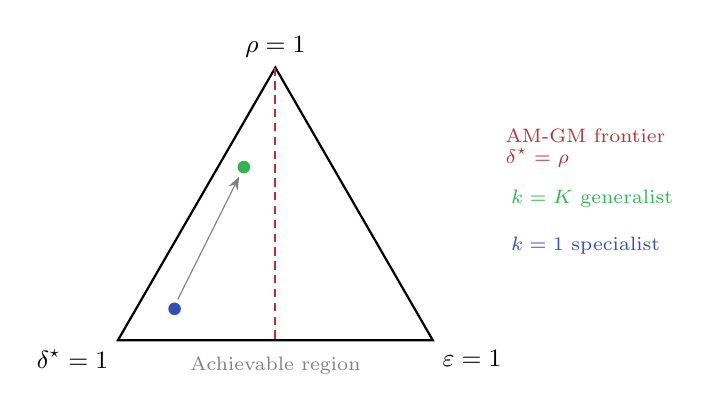
\begin{tikzpicture}[scale=4.0, >=Stealth]
\coordinate (A) at (0, 0);
\coordinate (B) at (1, 0);
\coordinate (C) at (0.5, 0.866);
\draw[thick] (A) -- (B) -- (C) -- cycle;
\node[below left, font=\small] at (A) {$\delta^\star = 1$};
\node[below right, font=\small] at (B) {$\varepsilon = 1$};
\node[above, font=\small] at (C) {$\rho = 1$};
\coordinate (M) at (0.5, 0);
\draw[densely dashed, mode1col, thick] (C) -- (M);
\node[mode1col, font=\scriptsize, right] at (1.2, 0.65) {AM-GM frontier};
\node[mode1col, font=\scriptsize, right] at (1.2, 0.58) {$\delta^\star = \rho$};
\fill[mode2col] (0.18, 0.10) circle (0.02);
\node[mode2col, font=\scriptsize, right=2pt] at (1.2, 0.30) 
    {$k = 1$ specialist};
\fill[mode3col] (0.40, 0.55) circle (0.02);
\node[mode3col, font=\scriptsize, right=2pt] at (1.2, 0.45)
    {$k = K$ generalist};
\draw[->, gray, thin] (0.19, 0.13) -- (0.385, 0.52);
\node[gray, font=\scriptsize] at (0.5, -0.08) {Achievable region};
\end{tikzpicture}
\caption{The reliability simplex. Vertices: pure robustness ($\dstar=1$), pure capacity ($\varrho=1$), pure slack ($\varepsilon=1$). The dashed median is the AM-GM frontier $\dstar = \varrho$. A $k=1$ specialist sits high in $\dstar$ and low in $\varrho$; a $k=K$ generalist trades $\dstar$ for $\varrho$. The product $\dstar\cdot\varrho$ is maximised on the median.}
\label{fig:simplex}
\end{figure}

The RP expresses the trade-off between robustness and capacity in any code: increasing $\varrho$ (the fraction of the parameter space used to encode information) forces $\dstar$ (the fraction available for error correction) downward, modulo the slack $\varepsilon$ absorbed by the architecture. The trade-off is structural, not imposed by any particular instantiation of the code.

\paragraph{Closing remark.}
Theorems~\ref{thm:jup} and~\ref{thm:rup} are independent: the JUP is a statement about the precision of dictionary-based identification at fixed code parameters, while the RP is a statement about the code parameters themselves. Together they give the two principal limits on diagnostic accuracy in the continuous syndrome algebra.

\newpage

\appendix

%==============================================================================
\section{Correspondence Table}
\label{app:correspondence}
%==============================================================================

The following table gives the complete structural correspondence between the discrete quantum code over $\Fbb_q$ and the continuous syndrome algebra over $\Rbb$. Each row records one structural component; the discrete column lists the $[\![5,1,3]\!]_2$ instantiation, and the continuous column lists the analogue established in this paper.

\begin{center}
\renewcommand{\arraystretch}{1.35}
\begin{tabular}{p{6.0cm}p{6.4cm}}
\toprule
\textbf{Discrete code (binary)} &
\textbf{Continuous syndrome algebra} \\
\midrule
Five physical qubits $(\Cnumber^2)^{\otimes 5}$ &
Parameter space $\Theta\subset\Rbb^n$ \\

One logical qubit ($k = 1$) &
One encoded domain ($k = 1$, optimal) \\

Minimum distance $d = 3$ &
Minimum number of simultaneously corrupted SVD directions \\

\mbox{Correction capacity} \mbox{$t = \lfloor (d-1)/2\rfloor = 1$} &
Same: single-direction errors are correctable \\

Alphabet $\Fbb_2$ ($q = 2$) &
Real field $\Rbb$ ($q\to\infty$) \\

Pauli operators $\{X_j, Z_j, Y_j\}$ &
SVD directions $\{\vk[k]\}$ \\

Symplectic form $\omega$ on $\Fbb_2^{10}$ &
Gram metric $\Gm = \Wm^\top\Wm$ on $\Rbb^{\dimin}$ \\

Four stabilizer generators $g_1,\dots,g_4$ &
Layers/measurement points $L\geq k^*$ \\

One generator $\to$ one syndrome bit &
One layer $\to$ one $d_L$-dimensional vector \\

All four generators $\to$ complete syndrome &
All layers $\to$ complete multi-layer syndrome \\

Parity-check matrix $\Hm \in \Fbb_2^{4\times 10}$ &
Averaged Jacobian $\bar{\Jm} \in \Rbb^{q\times\dimin}$ \\

Syndrome $\sk = \Hm\ek \pmod 2$ &
Syndrome table $\Sm = \Nop(\bar{\Jm}\cdot\Vm)^\top$ \\

Syndrome lookup by bitstring match &
Syndrome lookup by cosine maximisation \\

Inverse Pauli correction $E^{-1} = E$ &
Inverse perturbation $\Wm \mapsto \Wm - \varepsilon\uk[k]\vk[k]^\top$ \\

Undetectable: logical operator subspace &
Undetectable: null space $\mathcal{N}(\Wm)$ (Theorem~\ref{thm:null}) \\

Heisenberg bound (orthogonality) &
JUP (Theorem~\ref{thm:jup}) \\

Hamming bound saturated &
RP frontier (Theorem~\ref{thm:rup}) \\

\bottomrule
\end{tabular}
\end{center}

\newpage

%==============================================================================
\section{Worked Example: Discrete and Continuous Side by Side}
\label{app:worked}
%==============================================================================

This appendix works the same numerical situation through both the discrete $[\![5,1,3]\!]_2$ formalism and the continuous syndrome algebra, step by step. The reader can verify every entry by hand.

\subsection{The Discrete Case: \texorpdfstring{$X_3$}{X3} Error on Qubit 3}
\label{sec:appB_discrete}

\paragraph{Setup.}
Take the error operator $E = X_3$, a bit-flip on qubit~$3$. Its symplectic representation is
\[
  \ek \;=\; (a\,|\,b)
       \;=\; (0,0,1,0,0\,|\,0,0,0,0,0) \;\in\; \Fbb_2^{10}.
\]

\paragraph{Syndrome computation.}
The syndrome is $\sk = \Hm\ek \pmod 2$, with $\Hm$ given by \eqref{eq:hmatrix} and the symplectic pairing rule \eqref{eq:symplectic_rule}. The single non-zero entry of $\ek$ is at position~$3$ of the $a$-part, so the syndrome equals the $b$-coupling of position~$3$ across all generators:
\begin{align*}
  s_1 &= b_{g_1,\,3} \cdot a_{e,\,3} \;=\; 1\cdot 1 \;=\; 1
       \quad &&\text{(since $g_1$ has $Z$ at position $3$)} \\
  s_2 &= b_{g_2,\,3} \cdot a_{e,\,3} \;=\; 1\cdot 1 \;=\; 1
       \quad &&\text{(since $g_2$ has $Z$ at position $3$)} \\
  s_3 &= b_{g_3,\,3} \cdot a_{e,\,3} \;=\; 0\cdot 1 \;=\; 0
       \quad &&\text{(since $g_3$ has $X$ at position $3$, not $Z$)} \\
  s_4 &= b_{g_4,\,3} \cdot a_{e,\,3} \;=\; 0\cdot 1 \;=\; 0
       \quad &&\text{(since $g_4$ has $I$ at position $3$)}
\end{align*}
Hence $\sk = (1, 1, 0, 0) = \mathtt{1100}$.

\paragraph{Lookup and correction.}
Consulting Table~\ref{tab:syndromes513}, the syndrome $\mathtt{1100}$ corresponds to the error $X_3$. The correction is the application of $X_3$ again to the received state; since $X_3{}^2 = I$, the corruption is undone. Output: the original encoded state, exactly restored.

\subsection{The Continuous Case: SVD Direction \texorpdfstring{$\vk[3]$}{v3} Perturbation}
\label{sec:appB_continuous}

\paragraph{Setup.}
Take a small explicit weight matrix
\[
  \Wm \;=\; \begin{pmatrix}
    2 & 0 & 0 & 0 \\
    0 & 1.5 & 0 & 0 \\
    0 & 0 & 1 & 0 \\
    0 & 0 & 0 & 0.5
  \end{pmatrix} \in \Rbb^{4\times 4}.
\]
The SVD is immediate: $\Wm = \Imat_4 \cdot \mathrm{diag}(2, 1.5, 1, 0.5) \cdot \Imat_4^\top$, so $\Um = \Vm = \Imat_4$ and the singular values are $(\sigma_1, \sigma_2, \sigma_3, \sigma_4) = (2, 1.5, 1, 0.5)$. The SVD directions are the standard basis vectors:
\[
  \vk[1] = (1,0,0,0)^\top,\;\;
  \vk[2] = (0,1,0,0)^\top,\;\;
  \vk[3] = (0,0,1,0)^\top,\;\;
  \vk[4] = (0,0,0,1)^\top.
\]

\paragraph{The error operator.}
Since $\Wm$ is diagonal, $\Um = \Vm = \Imat_4$, so $\uk[k] = \vk[k]$ for every $k$. The SVD-aligned error operator in direction $k=3$ at magnitude $\varepsilon = 1.0$ is
\[
  \Delta\Wm_3(1.0) \;=\; 1.0\cdot \uk[3]\,\vk[3]^\top
  \;=\; \begin{pmatrix}0\\0\\1\\0\end{pmatrix}
        \begin{pmatrix}0 & 0 & 1 & 0\end{pmatrix}
  \;=\; \begin{pmatrix}
    0 & 0 & 0 & 0 \\
    0 & 0 & 0 & 0 \\
    0 & 0 & 1 & 0 \\
    0 & 0 & 0 & 0
  \end{pmatrix} .
\]
This is a rank-one matrix supported only in entry $(3,3)$: the perturbation shifts $\sigma_3 = 1$ to $\sigma_3 + \varepsilon = 2$ while leaving the other singular values, the left singular vectors, and the right singular vectors unchanged. The perturbed weight matrix is $\Wm' = \Wm + \Delta\Wm_3(1.0)$.

\paragraph{The logit map.}
Take the simplest possible logit: $\ell(x; \Wm) = \Wm x$, with $q = \dimout = 4$, $\dimin = 4$, and input $x\in\Rbb^4$. The first-order change in $\ell$ under the SVD-aligned perturbation $\Delta\Wm_k = \varepsilon\uk[k]\vk[k]^\top$ is
\[
  \ell(x;\Wm+\Delta\Wm_k) - \ell(x;\Wm)
  \;=\; \Delta\Wm_k\, x
  \;=\; \varepsilon\,(\vk[k]^\top x)\,\uk[k] .
\]
Reading off the Jacobian map $\vk[k] \mapsto \Jm(x)\vk[k]$ defined implicitly by~\eqref{eq:proof_taylor},
\[
  \Jm(x)\vk[k] \;=\; (\vk[k]^\top x)\,\uk[k] \quad\in\Rbb^4 .
\]
The Jacobian sends an input-space direction $\vk[k]$ to an output-space direction $\uk[k]$, scaled by the projection of the input onto $\vk[k]$.

\paragraph{Probe inputs and averaged Jacobian.}
Take $n_p = 3$ probes:
\[
  x_1 = (1, 1, 1, 1)^\top,\;\;
  x_2 = (1, 1, 1, 0)^\top,\;\;
  x_3 = (0, 1, 1, 1)^\top .
\]
The mean probe is $\bar{x} = (2/3,\,1,\,1,\,2/3)^\top$. For each $k$,
\[
  \bar{\Jm}\vk[k]
  \;=\; \frac{1}{n_p}\sum_i (\vk[k]^\top x_i)\,\uk[k]
  \;=\; (\vk[k]^\top \bar{x})\,\uk[k] ,
\]
giving $\bar{\Jm}\vk[1] = \tfrac{2}{3}\uk[1]$, $\bar{\Jm}\vk[2] = \uk[2]$, $\bar{\Jm}\vk[3] = \uk[3]$, $\bar{\Jm}\vk[4] = \tfrac{2}{3}\uk[4]$. All four projections $\vk[k]^\top \bar{x}$ are non-zero, so normalisation is well-defined and gives the syndrome
\[
  \sk[k] \;=\; \Nop(\bar{\Jm}\vk[k]) \;=\; \uk[k] .
\]
Stacking the syndromes as rows,
\[
  \Sm \;=\; \Nop(\bar{\Jm}\cdot\Vm)^\top \;=\; \Um^\top \;=\; \Imat_4
  \;\in\;\Rbb^{4\times 4} .
\]
The syndrome of the $k$-th SVD direction is the $k$-th left singular vector. In this diagonal example $\Um = \Imat_4$, so each syndrome is itself: the table is the identity. This is the continuous analogue of the discrete identity $\Sm = \Hm^\top$ for the $[\![5,1,3]\!]_2$ code (where $\Vm = \Imat$).

\paragraph{Identification.}
Suppose a test perturbation in direction $\vk[3]$ at unknown magnitude $\varepsilon_{\mathrm{test}}$ is applied. Pick a test input, say $x_{\mathrm{test}} = (1, 1, 1, 1)^\top$. The observed output change is
\[
  \boldsymbol{\delta}_{\mathrm{obs}}
  \;=\; \ell(x_{\mathrm{test}}; \Wm + \varepsilon_{\mathrm{test}}\uk[3]\vk[3]^\top)
       - \ell(x_{\mathrm{test}}; \Wm)
  \;=\; \varepsilon_{\mathrm{test}}\,(\vk[3]^\top x_{\mathrm{test}})\,\uk[3]
  \;=\; \varepsilon_{\mathrm{test}}\,\uk[3] .
\]
Therefore $\Nop(\boldsymbol{\delta}_{\mathrm{obs}}) = \uk[3]$. Compute cosine similarity with each row of $\Sm$:
\[
  \inner{\sk[k]}{\Nop(\boldsymbol{\delta}_{\mathrm{obs}})}
  \;=\; \inner{\uk[k]}{\uk[3]}
  \;=\; \delta_{k,3} .
\]
The argmax is $k = 3$, identified with cosine $1.000$. The magnitude estimate is $\varepsilon^* = \norm{\boldsymbol{\delta}_{\mathrm{obs}}} / \norm{\bar{\Jm}\vk[3]} = \varepsilon_{\mathrm{test}} / 1 = \varepsilon_{\mathrm{test}}$ for this probe-input configuration.

\paragraph{Correction.}
Apply $\Wm \mapsto \Wm + \varepsilon_{\mathrm{test}}\uk[3]\vk[3]^\top - \varepsilon^*\uk[3]\vk[3]^\top$ to undo. With $\varepsilon^* = \varepsilon_{\mathrm{test}}$ the correction is exact: $\Wm_{\mathrm{corrected}} = \Wm$ and the output is restored on every input. With a probe-induced estimation error $\Delta\varepsilon = \varepsilon^* - \varepsilon_{\mathrm{test}}$ the residual is $\ell(x;\Wm_{\mathrm{corrected}}) - \ell(x;\Wm) = \Delta\varepsilon\,(\vk[3]^\top x)\,\uk[3]$, linear in the magnitude mismatch.

\subsection{Side-by-Side Comparison}
\label{sec:appB_compare}

\begin{center}
\renewcommand{\arraystretch}{1.4}
\begin{tabular}{p{2.4cm} p{5.6cm} | p{5.6cm}}
\toprule
\textbf{Step} & \textbf{Discrete $[\![5,1,3]\!]_2$} &
\textbf{Continuous \mbox{syndrome algebra}} \\
\midrule
Setup &
\mbox{$X_3$ error on qubit 3;} \mbox{symplectic rep.\ $(0,0,1,0,0\,|\,\mathbf{0})$} &
\mbox{$\Delta\Wm_3(1.0) = \uk[3]\vk[3]^\top$;}
\mbox{SVD basis $\Vm = \Imat_4$, $\sigma_3 = 1$} \\
\midrule
Error basis &
\mbox{Pauli operators} \mbox{(standard basis in $\Fbb_2^{10}$)} &
SVD directions $\{\vk[1],\ldots,\vk[4]\}$ \\
\midrule
Parity-check / Jacobian &
$\Hm\in\Fbb_2^{4\times 10}$, eq.~\eqref{eq:hmatrix} &
\mbox{$\bar{\Jm} = \mathrm{diag}(2/3,\,1,\,1,\,2/3)$} \mbox{(this example)} \\
\midrule
Syndrome &
$\sk = \Hm\ek\pmod 2 = (1,1,0,0)^\top$ &
$\Sm = \Nop(\bar{\Jm}\cdot\Vm)^\top = \Imat_4$ \\
\midrule
Lookup &
Bitstring \texttt{1100} $\mapsto X_3$ (Table~\ref{tab:syndromes513}) &
$\mathrm{argmax}_k\inner{\sk[k]}{\boldsymbol{\delta}_{\mathrm{obs}}} = 3$ \\
\midrule
Correction &
Apply $X_3$ (Pauli self-inverse): $\Imat\to X_3 X_3\Imat = \Imat$ &
Apply $-\varepsilon^*\uk[3]\vk[3]^\top$: $\Wm' \to \Wm$ \\
\midrule
Field \mbox{arithmetic} &
$\pmod 2$: $1+1 = 0$, $1\cdot 1 = 1$ &
$\Rbb$: real-valued, cosines in $[-1, 1]$ \\
\bottomrule
\end{tabular}
\end{center}

\paragraph{The reduction map, made explicit.}
Setting in the continuous formula~\eqref{eq:main_thm}:
\begin{itemize}[nosep]
  \item $q = 2$ (binary alphabet)
  \item $\bar{\Jm} \leftarrow \Hm$ (sharp anticommutation, values
    in $\{0,1\}$)
  \item $\Vm = \Imat_{10}$ (Pauli basis equals standard basis in
    symplectic representation)
  \item $\Nop = \mathrm{id}$ (normalisation trivial in $\Fbb_2$)
  \item Inner product $\leftarrow$ bitstring AND, summed mod $2$
\end{itemize}
gives $\Sm = (\Hm \cdot \Imat_{10})^\top \pmod 2 = \Hm^\top \pmod 2$,
the $[\![5,1,3]\!]_2$ syndrome lookup table.

This concludes the worked example. The same construction works verbatim in the general continuous setting; the only difference is that $\Vm \neq \Imat$, $\bar{\Jm}$ takes values in $\Rbb$, and $\Nop$ is non-trivial. The reduction map shows that the discrete code is not merely analogous to the continuous algebra: it is the special case obtained by restricting the alphabet to $\Fbb_2$ and the basis to the Pauli basis.

\paragraph{Concerning applicability.}
The general validity of this construction --- and in particular whether it gives meaningful diagnostic information on a particular class of probabilistic systems --- is an empirical matter beyond the scope of the present mathematical paper. The companion paper \cite{ThreeModesLLM} demonstrates that the algebra developed here applies to a specific class of differentiable probabilistic systems whose parameter space is the weight space of a layered neural network, and reports numerical validation of every theorem proved above.

\newpage

\begin{thebibliography}{99}

\bibitem{ThreeModesLLM}
M.~Hubka, \emph{Three Measurable Failure Modes of Large Language Models}, 10.5281/zenodo.20127318 (2026)

\bibitem{Laflamme1996}
R.~Laflamme, C.~Miquel, J.~P.~Paz, and W.~H.~Zurek, \emph{Perfect quantum error correcting code}, Phys.\ Rev.\ Lett.\ \textbf{77} (1996), 198--201.

\bibitem{Bennett1996}
C.~H.~Bennett, D.~P.~DiVincenzo, J.~A.~Smolin, and W.~K.~Wootters, \emph{Mixed-State Entanglement and Quantum Error Correction}, \emph{Phys.\ Rev.\ A} \textbf{54}(5), 3824--3851 (1996).

\bibitem{Knill1997}
E.~Knill and R.~Laflamme, \emph{Theory of quantum error-correcting codes}, \emph{Phys.\ Rev.\ A} \textbf{55}(2), 900--911 (1997).

\bibitem{Singleton1964}
R.~C.~Singleton,
\emph{Maximum distance $q$-nary codes}, \emph{IEEE Trans.\ Inf.\ Theory} \textbf{10}(2), 116--118 (1964).

\bibitem{Ekert1996}
A.~Ekert and C.~Macchiavello, \emph{Quantum error correction for communication}, \emph{Phys.\ Rev.\ Lett.} \textbf{77}(12), 2585--2588 (1996).

\bibitem{NielsenChuang2000}
M.~A.~Nielsen and I.~L.~Chuang, \emph{Quantum Computation and Quantum Information}, Cambridge University Press (2000).

\bibitem{Gottesman1997}
D.~Gottesman, \emph{Stabilizer Codes and Quantum Error Correction}, Ph.D.\ thesis, California Institute of Technology (1997).

\bibitem{Horn2012}
R.~A.~Horn and C.~R.~Johnson, \emph{Matrix Analysis}, 2nd ed., Cambridge University Press, 2012.

\bibitem{Robertson1929}
H.~P.~Robertson, \emph{The uncertainty principle}, Phys.\ Rev.\ \textbf{34} (1929), 163--164.

\end{thebibliography}

\end{document}
